
%% bare_conf.tex
%% V1.4a
%% 2014/09/17
%% by Michael Shell
%% See:
%% http://www.michaelshell.org/
%% for current contact information.
%%
%% This is a skeleton file demonstrating the use of IEEEtran.cls
%% (requires IEEEtran.cls version 1.8a or later) with an IEEE
%% conference paper.
%%
%% Support sites:
%% http://www.michaelshell.org/tex/ieeetran/
%% http://www.ctan.org/tex-archive/macros/latex/contrib/IEEEtran/
%% and
%% http://www.ieee.org/

%%*************************************************************************
%% Legal Notice:
%% This code is offered as-is without any warranty either expressed or
%% implied; without even the implied warranty of MERCHANTABILITY or
%% FITNESS FOR A PARTICULAR PURPOSE! 
%% User assumes all risk.
%% In no event shall IEEE or any contributor to this code be liable for
%% any damages or losses, including, but not limited to, incidental,
%% consequential, or any other damages, resulting from the use or misuse
%% of any information contained here.
%%
%% All comments are the opinions of their respective authors and are not
%% necessarily endorsed by the IEEE.
%%
%% This work is distributed under the LaTeX Project Public License (LPPL)
%% ( http://www.latex-project.org/ ) version 1.3, and may be freely used,
%% distributed and modified. A copy of the LPPL, version 1.3, is included
%% in the base LaTeX documentation of all distributions of LaTeX released
%% 2003/12/01 or later.
%% Retain all contribution notices and credits.
%% ** Modified files should be clearly indicated as such, including  **
%% ** renaming them and changing author support contact information. **
%%
%% File list of work: IEEEtran.cls, IEEEtran_HOWTO.pdf, bare_adv.tex,
%%                    bare_conf.tex, bare_jrnl.tex, bare_conf_compsoc.tex,
%%                    bare_jrnl_compsoc.tex, bare_jrnl_transmag.tex
%%*************************************************************************


% *** Authors should verify (and, if needed, correct) their LaTeX system  ***
% *** with the testflow diagnostic prior to trusting their LaTeX platform ***
% *** with production work. IEEE's font choices and paper sizes can       ***
% *** trigger bugs that do not appear when using other class files.       ***                          ***
% The testflow support page is at:
% http://www.michaelshell.org/tex/testflow/



\documentclass[conference]{IEEEtran}
% Some Computer Society conferences also require the compsoc mode option,
% but others use the standard conference format.
%
% If IEEEtran.cls has not been installed into the LaTeX system files,
% manually specify the path to it like:
% \documentclass[conference]{../sty/IEEEtran}




% ------------- Packages Used --------------------------------------------------
% They help us to produce a better looking document ;-)
% ------------------------------------------------------------------------------

% Comment the following line before compiling the final version
%\synctex
\usepackage{multirow}

\usepackage{graphicx}
\usepackage{alltt}
\usepackage{relsize}
%\usepackage{xspace}
\usepackage{booktabs}
\usepackage{amsmath}
%\usepackage{multirow}
%\usepackage{array}
\usepackage{verbatim}
\usepackage[table]{xcolor}
\usepackage{caption}
\usepackage[labelformat=simple, labelsep=colon]{subcaption}{}
\captionsetup{compatibility=false}

%\usepackage[tight,footnotesize]{subfigure}

%\usepackage{capt-of}
%\usepackage{pifont}
\usepackage{amsfonts}
\usepackage{amssymb}
%\usepackage[latin1]{inputenc}
%\usepackage{times}
%\usepackage{colortbl}
%\usepackage{boxedminipage}
\usepackage{float}
%\usepackage{cite}
%\usepackage{fancyvrb}
%\usepackage{hyperref}
%\usepackage{balance}
\usepackage{url}
\usepackage{fancybox}%for \hypobox
\usepackage{listings}
\usepackage{array}
\usepackage{graphicx}
\usepackage{float}
%\usepackage{placeins}
\usepackage{multirow}
%\usepackage{blindtext}
%\usepackage{lipsum}
\usepackage{graphicx}
\usepackage{float}
%\usepackage{placeins}
\usepackage{multirow}
%\usepackage{caption} 

	
%\usepackage{subcaption}
%\usepackage{blindtext}
%\usepackage{lipsum}
\usepackage{graphicx}
\usepackage{amsmath}
\usepackage{booktabs}
\usepackage{framed}
\usepackage{multirow}% http://ctan.org/pkg/multirow
\usepackage{hhline}% http://ctan.org/pkg/hhline
\usepackage{amssymb}% http://ctan.org/pkg/amssymb
\usepackage{pifont}% http://ctan.org/pkg/pifont
\newcommand{\cmark}{\ding{51}}%
\newcommand{\xmark}{\ding{55}}%
%\usepackage{makecell}
%\usepackage{tablefootnote}

%\usepackage{textcomp}
%\usepackage{latexsym}
%\usepackage{amssymb}
%\usepackage{stmaryrd}
%\usepackage{euscript}
%\usepackage{wasysym}
%\usepackage{pifont}
%\usepackage{manfnt}
%\usepackage{undertilde}
%\usepackage{ifsym}
%\usepackage{tipa}
%\usepackage{txfonts}
%\usepackage{skak}
%\usepackage{skull}
%\usepackage{eurosym}
%\usepackage{yfonts}
%\usepackage{mathdots}
%\usepackage{trsym}
%\usepackage{upgreek}
%\usepackage{chemarr}
%\usepackage{accents}
%\usepackage{nicefrac}
%\usepackage{bm}


%\usepackage{pdfsync}

%   ACM Style
%\usepackage{lcsect}
% ------------------------------------------------------------------------------






% ------------ Color Definitions -----------------------------------------------
% Whatever colors we need
% ------------------------------------------------------------------------------
\definecolor{mygray}{rgb}{0.7,0.7,0.7}
% ------------------------------------------------------------------------------






% ---------- Special commands for annotating the paper's text ------------------
\let\mymarginpar\marginparm
\marginparwidth=1cm
\marginparsep=5pt
\newcommand{\todo}[1]{\textcolor{red}{\textbf{[[#1]]}}}
\def\TODO#1{\noindent\colorbox{yellow}{\bf \textcolor{red}{TODO: #1}}}
\newcommand{\hint}[1]{\textcolor{blue}{\textbf{#1}}}
\def\fig#1{Figure~\ref{#1}}
\def\tab#1{Table~\ref{#1}}
\def\eqn#1{Equation~\ref{#1}}
\def\sec#1{Section~\ref{#1}}

\pagenumbering{arabic}
\newcommand{\reviewer}[1]{\textcolor{DeepPink1}{{\it [Reviewer says: #1]}}}
\newcommand{\mei}[1]{\textcolor{red}{{\it [Mei says: #1]}}}
\newcommand{\ian}[1]{\textcolor{blue}{{\it [Ian says: #1]}}}
\newcommand{\nic}[1]{\textcolor{WildStrawberry}{{\it [Nico says: #1]}}}
\newcommand{\ahmed}[1]{\textcolor{green}{{\it [Ahmed says: #1]}}}
\newcommand{\myfoot}[1]{\footnote{\scriptsize #1}}
\newcommand{\myurl}[1]{\myfoot{\url{#1}}}
\newcommand{\Ra}{{$\Rightarrow$}}
\newcommand{\ra}{{$\rightarrow$}}
\newcommand{\La}{{$\Leftarrow$}}
\newcommand{\la}{{$\leftarrow$}}
\newcommand{\lra}{{$\leftrightarrow$}}
\newcommand{\LRa}{{$\Leftrightarrow$}}
%\newcommand{\todo}{\bram{todo}}

\newenvironment{myindentpar}[1]%
{\begin{list}{}%
         {\setlength{\leftmargin}{#1}}%
         \item[]%
}
{\end{list}}

% \AtBeginDocument{%
%    \renewcommand{\figurename}{Figure}%
%    \newcommand{\subfigureautorefname}{\figureautorefname}%for using subfig
% %   \renewcommand{\tablename}{TABLE}%
%    \renewcommand{\tablename}{Table}%
%    \renewcommand{\subsectionautorefname}{Section}%
%    \renewcommand{\sectionautorefname}{Section}%
% }

% Hypothesis box	
% ------------------------------------------------------------------------------	
\newcommand{\hypobox}[1]{\begin{center}%	
	\noindent\thicklines\setlength{\fboxsep}{7pt}%	
	\cornersize{0}\Ovalbox{\begin{minipage}{4.1in}%	
	\vspace{-0.1cm}
	\textit{#1}
	\vspace{-0.1cm}
	\end{minipage}} \end{center}}	
% ------------------------------------------------------------------------------




% ------------------------- SYMBOLS OF SELF NAMES OFTEN USED -------------------
\newcommand{\APACHE}{{\small APACHE}\xspace}
\newcommand{\BUGZILLA}{{\small BUGZILLA}\xspace}
\newcommand{\ECLIPSE}{{\small ECLIPSE}\xspace}
\newcommand{\ASPECTJ}{{\small ASPECTJ}\xspace}
\newcommand{\JDT}{{\small JDT}\xspace}
\newcommand{\GNU}{{\small GNU}\xspace}
\newcommand{\MOZILLA}{{\small MOZILLA}\xspace}
\newcommand{\THUNDERBIRD}{{\small THUNDERBIRD}\xspace}
\newcommand{\JAVA}{{\small Java}\xspace}
\newcommand{\GNOME}{{\small GNOME}\xspace}
\newcommand{\PG}{{\small PostgreSQL}\xspace}
\newcommand{\SIM}{{\small SimScan}\xspace}

% Anything else, e.g., \NAME{MICROSOFT}
\newcommand{\NAME}[1]{{\small #1}\xspace}
% ------------------------------------------------------------------------------




% ----------------------- Computer Science lol ---------------------------------
% Variable, function, and program names
% ------------------------------------------------------------------------------
\newcommand{\smalltt}[1]{\ifmmode{\mbox{\smaller\texttt{#1}}}\else{\smaller\tt #1}\fi}
\newcommand{\code}[1]{\smalltt{#1}}
\newcommand{\var}[1]{\code{#1}}
\newcommand{\func}[1]{\code{#1}}
\newcommand{\proc}[1]{\code{#1}}
\newcommand{\prog}[1]{\code{#1}}
\newcommand{\type}[1]{\code{#1}}
\newcommand{\progpt}[1]{\code{#1}}

\newcommand{\mypar}[1]{\vspace{.1cm}\noindent \textbf{#1}}
\newcommand{\myxpar}[1]{\vspace{.1cm}\noindent \textbf{#1}\newline}
% ------------------------------------------------------------------------------





% ----------- Things to remember -----------------------------------------------
\newenvironment{mynote}%
{ \medskip
  \noindent
  \let\emph=\textbf
  \begin{boxedminipage}{\columnwidth}\em}%
{ \end{boxedminipage}}
% ------------------------------------------------------------------------------






% -------------------- Use bars ------------------------------------------------
% These macros are for advanced presentation of results by shaded bars only!
% © Tom Zimmermann, 2008
% ------------------------------------------------------------------------------
\newdimen\qdx
\newdimen\qda
\newdimen\qdb
\def\rrrr#1#2#3#4{\newdimen\qd\qd=#4 % length of bar for 1.0
\qdx=\qd\multiply\qdx by 5\divide\qdx by 4
\qda=\qd
\qdb=\qd
\multiply\qda by #1\divide\qda by #3\multiply\qdb by #2\divide\qdb by #3\advance\qdb by -\qda
    \leavevmode\hbox to \qdx{\hfil\vbox{%
    \hbox{\vrule\vbox{\hrule\hbox to 1\qd
            {\vrule depth0pt height0.7ex width \qda\color{mygray}%
 \vrule depth0pt height0.7ex width \qdb\hfill}\hrule}\vrule}
    }\hfil}}
\def\rrr#1#2#3{\rrrr{#1}{#2}{#3}{0.8cm}}
% -------------------------------------------------------------------------






% ------------ Graphics Hacks --------------------------------------------------
% Use these settings if Figures tend to get their one separate pages
% ------------------------------------------------------------------------------
% \renewcommand{\topfraction}{0.85}
% \renewcommand{\textfraction}{0.1}
% \renewcommand{\floatpagefraction}{0.75}
% ------------------------------------------------------------------------------





% ------------------ Biblio Hack -----------------------------------------------
% Use these settings if the References take too much space
% ------------------------------------------------------------------------------
\let\oldthebibliography=\thebibliography
  \let\endoldthebibliography=\endthebibliography
  \renewenvironment{thebibliography}[1]{%
%	\vspace{-0.3cm}
    \begin{oldthebibliography}{#1}%
%	\vspace{-0.2cm}
       \setlength{\parskip}{0ex}%
       \setlength{\itemsep}{0ex}%
%	\bibfont
  }%
  {%
    \end{oldthebibliography}%
  }
% ------------------------------------------------------------------------------





% -------------- Floats Redefined ----------------------------------------------
% Use these settings to change the whitespace between floats and text
% ------------------------------------------------------------------------------

% \setlength\dblfloatsep{1pt}
% \setlength\floatsep{1pt}
% \setlength\textfloatsep{5pt}
% \setlength\dbltextfloatsep{5pt}

% \renewcommand\floatpagefraction{.9}
% \renewcommand\topfraction{.9}
% \renewcommand\bottomfraction{.9}
% \renewcommand\textfraction{.1}
% \setcounter{totalnumber}{50}
% \setcounter{topnumber}{50}
% \setcounter{bottomnumber}{50}
% ------------------------------------------------------------------------------
\makeatletter




% Some very useful LaTeX packages include:
% (uncomment the ones you want to load)


% *** MISC UTILITY PACKAGES ***
%
%\usepackage{ifpdf}
% Heiko Oberdiek's ifpdf.sty is very useful if you need conditional
% compilation based on whether the output is pdf or dvi.
% usage:
% \ifpdf
%   % pdf code
% \else
%   % dvi code
% \fi
% The latest version of ifpdf.sty can be obtained from:
% http://www.ctan.org/tex-archive/macros/latex/contrib/oberdiek/
% Also, note that IEEEtran.cls V1.7 and later provides a builtin
% \ifCLASSINFOpdf conditional that works the same way.
% When switching from latex to pdflatex and vice-versa, the compiler may
% have to be run twice to clear warning/error messages.






% *** CITATION PACKAGES ***
%
%\usepackage{cite}
% cite.sty was written by Donald Arseneau
% V1.6 and later of IEEEtran pre-defines the format of the cite.sty package
% \cite{} output to follow that of IEEE. Loading the cite package will
% result in citation numbers being automatically sorted and properly
% "compressed/ranged". e.g., [1], [9], [2], [7], [5], [6] without using
% cite.sty will become [1], [2], [5]--[7], [9] using cite.sty. cite.sty's
% \cite will automatically add leading space, if needed. Use cite.sty's
% noadjust option (cite.sty V3.8 and later) if you want to turn this off
% such as if a citation ever needs to be enclosed in parenthesis.
% cite.sty is already installed on most LaTeX systems. Be sure and use
% version 5.0 (2009-03-20) and later if using hyperref.sty.
% The latest version can be obtained at:
% http://www.ctan.org/tex-archive/macros/latex/contrib/cite/
% The documentation is contained in the cite.sty file itself.






% *** GRAPHICS RELATED PACKAGES ***
%
\ifCLASSINFOpdf
  % \usepackage[pdftex]{graphicx}
  % declare the path(s) where your graphic files are
  % \graphicspath{{../pdf/}{../jpeg/}}
  % and their extensions so you won't have to specify these with
  % every instance of \includegraphics
  % \DeclareGraphicsExtensions{.pdf,.jpeg,.png}
\else
  % or other class option (dvipsone, dvipdf, if not using dvips). graphicx
  % will default to the driver specified in the system graphics.cfg if no
  % driver is specified.
  % \usepackage[dvips]{graphicx}
  % declare the path(s) where your graphic files are
  % \graphicspath{{../eps/}}
  % and their extensions so you won't have to specify these with
  % every instance of \includegraphics
  % \DeclareGraphicsExtensions{.eps}
\fi
% graphicx was written by David Carlisle and Sebastian Rahtz. It is
% required if you want graphics, photos, etc. graphicx.sty is already
% installed on most LaTeX systems. The latest version and documentation
% can be obtained at: 
% http://www.ctan.org/tex-archive/macros/latex/required/graphics/
% Another good source of documentation is "Using Imported Graphics in
% LaTeX2e" by Keith Reckdahl which can be found at:
% http://www.ctan.org/tex-archive/info/epslatex/
%
% latex, and pdflatex in dvi mode, support graphics in encapsulated
% postscript (.eps) format. pdflatex in pdf mode supports graphics
% in .pdf, .jpeg, .png and .mps (metapost) formats. Users should ensure
% that all non-photo figures use a vector format (.eps, .pdf, .mps) and
% not a bitmapped formats (.jpeg, .png). IEEE frowns on bitmapped formats
% which can result in "jaggedy"/blurry rendering of lines and letters as
% well as large increases in file sizes.
%
% You can find documentation about the pdfTeX application at:
% http://www.tug.org/applications/pdftex





% *** MATH PACKAGES ***
%
%\usepackage[cmex10]{amsmath}
% A popular package from the American Mathematical Society that provides
% many useful and powerful commands for dealing with mathematics. If using
% it, be sure to load this package with the cmex10 option to ensure that
% only type 1 fonts will utilized at all point sizes. Without this option,
% it is possible that some math symbols, particularly those within
% footnotes, will be rendered in bitmap form which will result in a
% document that can not be IEEE Xplore compliant!
%
% Also, note that the amsmath package sets \interdisplaylinepenalty to 10000
% thus preventing page breaks from occurring within multiline equations. Use:
%\interdisplaylinepenalty=2500
% after loading amsmath to restore such page breaks as IEEEtran.cls normally
% does. amsmath.sty is already installed on most LaTeX systems. The latest
% version and documentation can be obtained at:
% http://www.ctan.org/tex-archive/macros/latex/required/amslatex/math/





% *** SPECIALIZED LIST PACKAGES ***
%
%\usepackage{algorithmic}
% algorithmic.sty was written by Peter Williams and Rogerio Brito.
% This package provides an algorithmic environment fo describing algorithms.
% You can use the algorithmic environment in-text or within a figure
% environment to provide for a floating algorithm. Do NOT use the algorithm
% floating environment provided by algorithm.sty (by the same authors) or
% algorithm2e.sty (by Christophe Fiorio) as IEEE does not use dedicated
% algorithm float types and packages that provide these will not provide
% correct IEEE style captions. The latest version and documentation of
% algorithmic.sty can be obtained at:
% http://www.ctan.org/tex-archive/macros/latex/contrib/algorithms/
% There is also a support site at:
% http://algorithms.berlios.de/index.html
% Also of interest may be the (relatively newer and more customizable)
% algorithmicx.sty package by Szasz Janos:
% http://www.ctan.org/tex-archive/macros/latex/contrib/algorithmicx/




% *** ALIGNMENT PACKAGES ***
%
%\usepackage{array}
% Frank Mittelbach's and David Carlisle's array.sty patches and improves
% the standard LaTeX2e array and tabular environments to provide better
% appearance and additional user controls. As the default LaTeX2e table
% generation code is lacking to the point of almost being broken with
% respect to the quality of the end results, all users are strongly
% advised to use an enhanced (at the very least that provided by array.sty)
% set of table tools. array.sty is already installed on most systems. The
% latest version and documentation can be obtained at:
% http://www.ctan.org/tex-archive/macros/latex/required/tools/


% IEEEtran contains the IEEEeqnarray family of commands that can be used to
% generate multiline equations as well as matrices, tables, etc., of high
% quality.




% *** SUBFIGURE PACKAGES ***
%\ifCLASSOPTIONcompsoc
%  \usepackage[caption=false,font=normalsize,labelfont=sf,textfont=sf]{subfig}
%\else
%  \usepackage[caption=false,font=footnotesize]{subfig}
%\fi
% subfig.sty, written by Steven Douglas Cochran, is the modern replacement
% for subfigure.sty, the latter of which is no longer maintained and is
% incompatible with some LaTeX packages including fixltx2e. However,
% subfig.sty requires and automatically loads Axel Sommerfeldt's caption.sty
% which will override IEEEtran.cls' handling of captions and this will result
% in non-IEEE style figure/table captions. To prevent this problem, be sure
% and invoke subfig.sty's "caption=false" package option (available since
% subfig.sty version 1.3, 2005/06/28) as this is will preserve IEEEtran.cls
% handling of captions.
% Note that the Computer Society format requires a larger sans serif font
% than the serif footnote size font used in traditional IEEE formatting
% and thus the need to invoke different subfig.sty package options depending
% on whether compsoc mode has been enabled.
%
% The latest version and documentation of subfig.sty can be obtained at:
% http://www.ctan.org/tex-archive/macros/latex/contrib/subfig/




% *** FLOAT PACKAGES ***
%
%\usepackage{fixltx2e}
% fixltx2e, the successor to the earlier fix2col.sty, was written by
% Frank Mittelbach and David Carlisle. This package corrects a few problems
% in the LaTeX2e kernel, the most notable of which is that in current
% LaTeX2e releases, the ordering of single and double column floats is not
% guaranteed to be preserved. Thus, an unpatched LaTeX2e can allow a
% single column figure to be placed prior to an earlier double column
% figure. The latest version and documentation can be found at:
% http://www.ctan.org/tex-archive/macros/latex/base/


%\usepackage{stfloats}
% stfloats.sty was written by Sigitas Tolusis. This package gives LaTeX2e
% the ability to do double column floats at the bottom of the page as well
% as the top. (e.g., "\begin{figure*}[!b]" is not normally possible in
% LaTeX2e). It also provides a command:
%\fnbelowfloat
% to enable the placement of footnotes below bottom floats (the standard
% LaTeX2e kernel puts them above bottom floats). This is an invasive package
% which rewrites many portions of the LaTeX2e float routines. It may not work
% with other packages that modify the LaTeX2e float routines. The latest
% version and documentation can be obtained at:
% http://www.ctan.org/tex-archive/macros/latex/contrib/sttools/
% Do not use the stfloats baselinefloat ability as IEEE does not allow
% \baselineskip to stretch. Authors submitting work to the IEEE should note
% that IEEE rarely uses double column equations and that authors should try
% to avoid such use. Do not be tempted to use the cuted.sty or midfloat.sty
% packages (also by Sigitas Tolusis) as IEEE does not format its papers in
% such ways.
% Do not attempt to use stfloats with fixltx2e as they are incompatible.
% Instead, use Morten Hogholm'a dblfloatfix which combines the features
% of both fixltx2e and stfloats:
%
% \usepackage{dblfloatfix}
% The latest version can be found at:
% http://www.ctan.org/tex-archive/macros/latex/contrib/dblfloatfix/




% *** PDF, URL AND HYPERLINK PACKAGES ***
%
%\usepackage{url}
% url.sty was written by Donald Arseneau. It provides better support for
% handling and breaking URLs. url.sty is already installed on most LaTeX
% systems. The latest version and documentation can be obtained at:
% http://www.ctan.org/tex-archive/macros/latex/contrib/url/
% Basically, \url{my_url_here}.




% *** Do not adjust lengths that control margins, column widths, etc. ***
% *** Do not use packages that alter fonts (such as pslatex).         ***
% There should be no need to do such things with IEEEtran.cls V1.6 and later.
% (Unless specifically asked to do so by the journal or conference you plan
% to submit to, of course. )


% correct bad hyphenation here
\hyphenation{op-tical net-works semi-conduc-tor}
%DIF PREAMBLE EXTENSION ADDED BY LATEXDIFF
%DIF UNDERLINE PREAMBLE %DIF PREAMBLE
\RequirePackage[normalem]{ulem} %DIF PREAMBLE
\RequirePackage{color}\definecolor{RED}{rgb}{1,0,0}\definecolor{BLUE}{rgb}{0,0,1} %DIF PREAMBLE
\providecommand{\DIFadd}[1]{{\protect\color{blue}\uwave{#1}}} %DIF PREAMBLE
\providecommand{\DIFdel}[1]{{\protect\color{red}\sout{#1}}}                      %DIF PREAMBLE
%DIF SAFE PREAMBLE %DIF PREAMBLE
\providecommand{\DIFaddbegin}{} %DIF PREAMBLE
\providecommand{\DIFaddend}{} %DIF PREAMBLE
\providecommand{\DIFdelbegin}{} %DIF PREAMBLE
\providecommand{\DIFdelend}{} %DIF PREAMBLE
%DIF FLOATSAFE PREAMBLE %DIF PREAMBLE
\providecommand{\DIFaddFL}[1]{\DIFadd{#1}} %DIF PREAMBLE
\providecommand{\DIFdelFL}[1]{\DIFdel{#1}} %DIF PREAMBLE
\providecommand{\DIFaddbeginFL}{} %DIF PREAMBLE
\providecommand{\DIFaddendFL}{} %DIF PREAMBLE
\providecommand{\DIFdelbeginFL}{} %DIF PREAMBLE
\providecommand{\DIFdelendFL}{} %DIF PREAMBLE
%DIF END PREAMBLE EXTENSION ADDED BY LATEXDIFF

\begin{document}
%
% paper title
% Titles are generally capitalized except for words such as a, an, and, as,
% at, but, by, for, in, nor, of, on, or, the, to and up, which are usually
% not capitalized unless they are the first or last word of the title.
% Linebreaks \\ can be used within to get better formatting as desired.
% Do not put math or special symbols in the title.
% Do not put math or special symbols in the title.
\title{An Empirical Study On Leveraging Logs During Bug Fixes}


% author names and affiliations
% use a multiple column layout for up to three different
% affiliations
\author{\IEEEauthorblockN{Suhas Kabinna, Weiyi Shang, Ahmed E. Hassan}
	\IEEEauthorblockA{School of Computing\\
		Queen's University\\
		Kingston, Ontario, Canada K7L 2N8\\
		Email: \{kabinna, swy, ahmed\}@queensu.ca}
}
% conference papers do not typically use \thanks and this command
% is locked out in conference mode. If really needed, such as for
% the acknowledgment of grants, issue a \IEEEoverridecommandlockouts
% after \documentclass

% for over three affiliations, or if they all won't fit within the width
% of the page, use this alternative format:
% 
%\author{\IEEEauthorblockN{Michael Shell\IEEEauthorrefmark{1},
%Homer Simpson\IEEEauthorrefmark{2},
%James Kirk\IEEEauthorrefmark{3}, 
%Montgomery Scott\IEEEauthorrefmark{3} and
%Eldon Tyrell\IEEEauthorrefmark{4}}
%\IEEEauthorblockA{\IEEEauthorrefmark{1}School of Electrical and Computer Engineering\\
%Georgia Institute of Technology,
%Atlanta, Georgia 30332--0250\\ Email: see http://www.michaelshell.org/contact.html}
%\IEEEauthorblockA{\IEEEauthorrefmark{2}Twentieth Century Fox, Springfield, USA\\
%Email: homer@thesimpsons.com}
%\IEEEauthorblockA{\IEEEauthorrefmark{3}Starfleet Academy, San Francisco, California 96678-2391\\
%Telephone: (800) 555--1212, Fax: (888) 555--1212}
%\IEEEauthorblockA{\IEEEauthorrefmark{4}Tyrell Inc., 123 Replicant Street, Los Angeles, California 90210--4321}}




% use for special paper notices
%\IEEEspecialpapernotice{(Invited Paper)}




% make the title area
\maketitle

% As a general rule, do not put math, special symbols or citations
% in the abstract
\begin{abstract}
	Logging is a practice leveraged by software developers to record and convey important 
	information during the execution of a system. Logs can be used to
	output the behavior of the system when running, to monitor the choke
	points of a system, and to help in debugging the system. These logs are valuable sources of information for developers in debugging large software systems. Prior research has shown that over 41\% of log changes are made during bug fixes. However, little is known about how logs are leveraged during bug fixes. In this paper, we sought to study the leverage of logs during bug fixes through case studies on three large open source systems namely  Hadoop, HBase and Qpid. We find that logs are changed \DIFdelbegin \DIFdel{a }\DIFdelend statistically significantly more in bug fixes than other code changes. Furthermore, we find four different types of log modifications that developers make to logging statements during bug fixes: (1)changes to logging level, (2)changes to the textual content of a log, (3)changes to logging parameters and (4)relocation of logs. \DIFdelbegin \DIFdel{We }\DIFdelend \DIFaddbegin \DIFadd{In addition we }\DIFaddend find that developers modify variables more during bug fixes\DIFaddbegin \DIFadd{, than adding or deleting logs}\DIFaddend .  Finally, we find that \DIFdelbegin \DIFdel{issue reports }\DIFdelend \DIFaddbegin \DIFadd{bug fixing commits }\DIFaddend with log changes have larger code churn, but involve fewer developers, require less time and have less discussion during the fix process. We  train a linear model and find that adding and modifying logging statements is \DIFdelbegin \DIFdel{statistically significant and reduce }\DIFdelend \DIFaddbegin \DIFadd{negatively co-related to }\DIFaddend the resolution time of bug fixes. \DIFdelbegin \DIFdel{These findings show that developer should leverage logs more in practice to fix }\DIFdelend \DIFaddbegin \DIFadd{This suggests that leveraging logs helps in the quicker resolution of }\DIFaddend bugs.
%	This shows that logs are helpful in quicker resolution of bugs and demonstrates the importance logs play in bug fixes and motivates developers to log more.
	%	bug fixes with log changes have larger code churn

	
	%	Though much research has been done on the analysis of logs, most of
	%	the studies looked at either characterizing logs based on their usage
	%	or how to improve logs so they are more meaningful. But, there has
	%	been no study so far which looks into how effective logs are in the
	%	software development process and especially in debugging. 
	%	
	%	To answer this question in our paper we first try to find co-relation
	%	between log updates and bug fixes. This is an intuitive step, because
	%	when developers fix bugs they update the logs associated with the
	%	bug or add new logs to help them fix bugs. We verify this claim on
	%	3 large scale systems 
	%	We then find the types of changes developers make to logging statements
	%	during bug fixes. Finally, we look at how long it takes for bugs to get fixed,
	%	the number of developers involved in the fix and the comments associated
	%	with the fixes, all with respect to bugs without logging changes.\\
	%	\indent We find that in all projects logging actually helps in the debugging
	%	process and three factors - time, developers and comments - are lesser
	%	when bugs have log churn associated with them.

\end{abstract}

% no keywords




% For peer review papers, you can put extra information on the cover
% page as needed:
% \ifCLASSOPTIONpeerreview
% \begin{center} \bfseries EDICS Category: 3-BBND \end{center}
% \fi
%
% For peerreview papers, this IEEEtran command inserts a page break and
% creates the second title. It will be ignored for other modes.
\IEEEpeerreviewmaketitle






\section{Introduction}


Logs \DIFaddbegin \DIFadd{are }\DIFaddend leveraged by developers to record useful information during the execution of a system. Logging can be done through simple \textsl{printf} statements or through  logging libraries such as `Log4j', `Slf4j', and `JCL'. Each log contains a textual part that gives information about the context, a variable part that contains information about the events, and \DIFdelbegin \DIFdel{logging levels }\DIFdelend \DIFaddbegin \DIFadd{a logging level }\DIFaddend that shows the verbosity of the logs.
%The 5 commonly used logging levels are 'DEBUG', 'INFO', 'WARN', 'ERROR', 'FATAL' and these help in %providing additional information about an event. 
An example of a logging statement is shown below where \emph{info} is the logging level, \emph{Connected to} is the event and the \DIFdelbegin \DIFdel{value of variable \emph{host} is the }\DIFdelend variable \DIFaddbegin \DIFadd{\emph{host} contains information about the event}\DIFaddend .

%The 5 commonly used logging levels are 'DEBUG', 'INFO', 'WARN', 'ERROR', 'FATAL' 
\hypobox{ \hspace{25pt} LOG.info( ``Connected to " + host);}
%\fbox{\begin{minipage}[t]{0.9\columnwidth}%
%LOG.info("Connected to " + host);%
%\end{minipage}}



Research has shown that logs are used by developers extensively
during the development of software systems~\cite{Characterizinglogs}. Logs are leveraged for detecting anomalies~\cite{XUanomalies,ConsoleLogs,Marksyer}, monitoring the performance of systems~\cite{Bitperformance}, maintenance of large systems~\cite{Marksyer}, capacity planning of large systems~\cite{IanWCRE} and debugging~\cite{EMSEIAN}. The valuable information in logs has created a new market for log maintenance platforms like Splunk~\cite{Bitperformance}, XpoLog~\cite{Xpolog}, and Logstash~\cite{Logstash}, which assist developers in analyzing logs.

Logs are also used extensively to help developers to fix \DIFdelbegin \DIFdel{bus  }\DIFdelend \DIFaddbegin \DIFadd{bugs  }\DIFaddend in large software systems.
%the development process. This is because the increasing complexity of software systems  makes it  difficult for developers to understand the
%functionality of every module, or to diagnose a system error.
  For example, in the JIRA issue HBASE-3403 (commit \DIFdelbegin \DIFdel{1056484}\DIFdelend \DIFaddbegin \DIFadd{1,056,484}\DIFaddend ), a bug is reported when a module does not exit upon system failure.\DIFdelbegin \DIFdel{In order to fix this bug, developers needed to  record more information in the existing logs}\DIFdelend \DIFaddbegin \DIFadd{To find the point of failure, developers leverage log data}\DIFaddend . After the \DIFdelbegin \DIFdel{bug was fixed, the added information in the logs has been used by developers }\DIFdelend \DIFaddbegin \DIFadd{fix, the logs or updated }\DIFaddend to prevent similar bugs in the system. 
%DIF >    In order to fix this bug, developers needed to  record more information in the existing logs. After the bug was fixed, the added information in the logs has been used by developers to prevent similar bugs in the system.
%we see that  developers try fixing a bug where a module does not exit after a failure.
%The developer provides logs in the description and explains that he
%will go through logs to understand how this particular was state was
%obtained.
%As the logs do not provide sufficient information, one of the developer mentions 
%As the logs fail to identify the root-cause of the bug. One of the
%developer mentioned
% \textit{' The log does not have important transition
%points for the above cited problematic region nor for the few that
%are stuck PENDING\_CLOSE on end of the log. Let me try reproduce'}. The bug is solved after 7 days and the logs are updated for future fixes.
%After spending 7 days to fix the bug, the developers update the old logging statements to assist in fixing future bugs.
%reproducing the bug in an unit tests, they manage to fix the
%bug. This bug being of 'Blocker' category (highest level) takes over
%7 days to get fixed. We also observe that they update the old logging
%statements during the fix so all future bugs in the segment can be
%resolved quickly. 

 Prior research performs a manual study on  bug fixes. The results show that 41\% of log changes are used to assist \DIFdelbegin \DIFdel{in }\DIFdelend debugging~\cite{EMSEIAN}. However, there exists no large scale empirical study of how logs are leveraged during bug fixes.
%This includes logs used in providing more information about control flow, recording events and also in debugging. 
%%n large scale systems like Cassandra, HBase, HDFS and Redis. There has been research
%%done where the logging practices are characterized based on the functions
%%they fulfill ~\cite{Characterizinglogs}. The functions can be to provide
%%information about control flow, to record events for tracing and also
%%to debug error. 
%
%Studies have been also done on large scale systems like Cassandra, HBase, HDFS and Redis to show the usefulness of logs in debugging process ~\cite{Simpletesting}. A manual study done before shows that 41\% of the log changes are done during bug fixes


%Most of the previous work was done on manual sampled analysis of systems.
%The test cases were done on a single project and no work has been
%to understand the leverage of logs during bug fixes in particular.
%One of the primary reasons is because, it is difficult to know when
%logs are being leveraged during bug fixes.

In this paper, we perform an empirical study on how logs are leveraged during the bug fixes of \DIFdelbegin \DIFdel{the }\DIFdelend Hadoop, HBase and Qpid \DIFaddbegin \DIFadd{projects}\DIFaddend . In particular, we sought to answer following research questions. 
% we first try to establish that logs are modified along
%with bugs. Previous research has shown that files which have high
%churn are more prone to defects ~\cite{NagappanBugpredictions,Nagappanmodulebug}.
%This means that developers also change logs also during bug fixes
%so that subsequent bugfixes are simpler. We explore such changes to
%logs through the help of the following research questions:


\begin{description}
\item[\textbf{RQ1:}]\textbf{Are logs leveraged more during bug fixes } 

We find that logs are leveraged more frequently during bug fixing \DIFdelbegin \DIFdel{changes }\DIFdelend \DIFaddbegin \DIFadd{commits }\DIFaddend than non-bug fixing \DIFdelbegin \DIFdel{changes}\DIFdelend \DIFaddbegin \DIFadd{commits}\DIFaddend . In particular, we find that log addition and log modification appear more in bug fixing commits than non-bug fixing commits, to a statistically significant degree, with non-trivial effect size. We identified 4 types of log modifications namely \em{`Logging level change', `Text Modification', `Variable Change'} and \em{Log Relocation'}. We find that \em{`Text Modification', `Variable Change'} and \em{`Relocating'} are statistically significant, with medium to high effect sizes in bug fixing commits. This shows that developers need specific information from logs to help fix bugs.

%This suggests that developers leverage logs during bug fixes.   
%The effect size \cite{Effectsize} was in the small range for log
%modifications in Hadoop and Qpid. We found that even log addition
%was in small range for Qpid. This shows that during bug fixing operations,
%logs are modified or added as they are closely related to the bug.
%It also shows that, developers have fair idea which modules can lead
%to bugs so they have log statements to assist them and later update
%them accordingly.

%\textbf{RQ2: What types of modifications  to logs are more frequent during bug fix?}
%
%We manually identified four types of log modifications from our case studies.
%The 4 types of changes are \em{'Logging level change', 'Text Modification', 'Variable Change'} and \em{'Relocating logs'}. We found that \em{'Text Modification', 'Variable Change'} and \em{'Relocating'} are statistically  more significant, with medium to high effect sizes in bug fixing commits. This shows that developers need specific information from logs can help fix bugs.	
\begin{figure*}
	\centering
	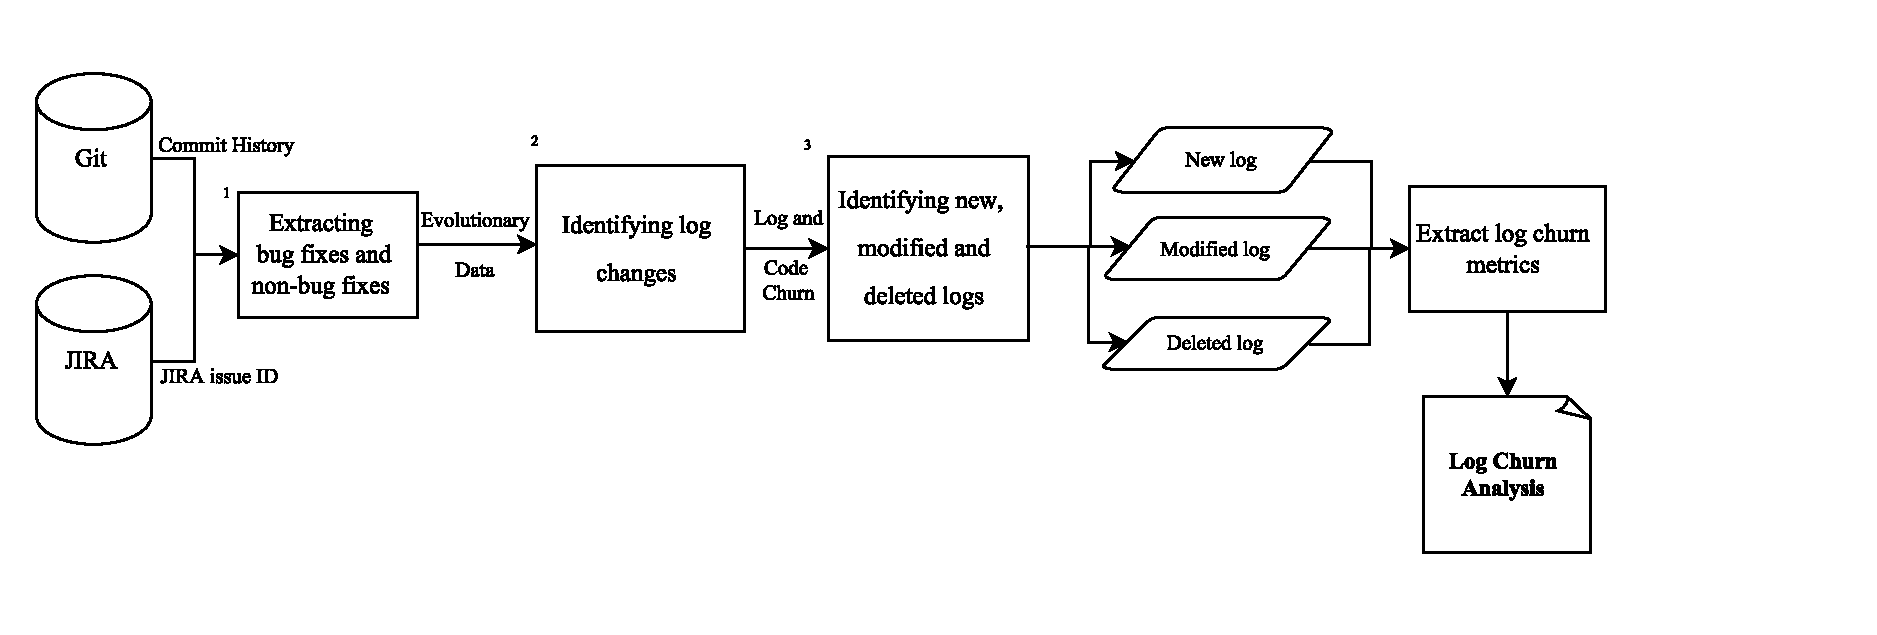
\includegraphics{MethdologyICESEM}
	\caption{ Overview of our cast study approach }
	\label{fig:MethodologyICSME}
\end{figure*}


\item[\textbf{RQ2:}]\textbf{	Are logs useful in bug fixes?}

We find that logs help in a faster resolution of bugs with less developer
involvement. We find that bug fixing commits with log changes have
higher code churn. This implies that logs are leveraged to fix more complex bugs. After controlling for code churn, we find that the issues with log changes take less time to get resolved, involve fewer \DIFdelbegin \DIFdel{developer }\DIFdelend \DIFaddbegin \DIFadd{developers }\DIFaddend and have less discussions during the bug fixing process. Using these metrics we trained a linear model to study the effect that log churn related metrics have on resolution time of bug fixes.
 We find that log churn related metrics are statistically significant in the model and have a negative effect on resolution time of bug fixes. This shows that developers should leverage logs more in practice to assist in the faster resolution of bugs.


\end{description}

%\textbf{RQ3: Does log churn impact resolution time of bug fixes?}
%\indent We found that log churn has negative impact on resolution time of bug fixes. In particular we found that  \textsl{'New Log churn'} and \textsl{'Modified Log churn'} have negative impact on resolution time and are statistically significant. This implies that adding and modifying logging statements during bug fixes, can help in reducing the resolution time for the bug fix.



\begin{table*}
		\protect\caption{An overview of the subject systems}
		\label{tba:Overview}
	\centering{}%
	\begin{tabular}{|>{\centering}p{3cm}|c|c|c|c|c|c|}
		\hline 
		\multirow{2}{*}{Projects} & \multicolumn{2}{c|}{Hadoop} & \multicolumn{2}{c|}{HBase} & \multicolumn{2}{c|}{Qpid}\tabularnewline
		\cline{2-7} 
		& Bug fixing  & Non-Bug Fixing & Bug fixing  & Non-Bug Fixing & Bug fixing  & Non-Bug Fixing \tabularnewline
		\hline 
		\# of Revisions & 7,366 & 12,300 & 5,149 & 7,784 & 1,824 & 5,684\tabularnewline
		\hline 
		Code Churn & 4,09K & 3.2M & 1.4M & 2.18M & 175k & 2.3M\tabularnewline
		\hline 
		Log Churn & 4,311 & 23,838 & 4,566 & 12,005 & 597 & 10,238\tabularnewline
		\hline 
	\end{tabular}
\end{table*}




%Finally, we performed a manual study where we sampled 255 buggy JIRA issues, with changes to logs to understand how logs are used in finding bugs. 
%%commits with log churn to understand the usefulness of logs. 
%We found that over 70\% of commits directly used logs to assist in the debugging
%process. Over 61\% of those used the textual and variable objects
%present in logs to help in the debugging process. We found that developers use the log information to understand the rationale behind the bugs and when more information is required, change logging statements.	 
% This study proved that logs are useful in the debugging process
%and developers tend to use logs to find the condition and rationale
%of bugs to help them in debugging. 
%
%Our study highlights that logs are useful in the debugging process
%and developers need to dedicate more time towards logging as and follow
%good logging practices.

The rest of this paper is organized as follows.  Section \DIFaddbegin \DIFadd{\ref{sec:Manual} presents a qualitative study  to motivate the paper. Section }\DIFaddend \ref{sec:Methodology}  presents the  methodology for gathering and extracting data for our study. Section \ref{sec:Study}  presents the  case studies and the results to answer the two research questions. Section \DIFdelbegin \DIFdel{\ref{sec:Manual} presents a manual analysis on bug fixing commits with log changes. Section }\DIFdelend \ref{sec:Related} describes the prior research that is related to our work. Section \ref{sec:Limit}  discusses the threats to validity. Finally section \ref{sec:Conclusion}  concludes the paper.




\DIFaddbegin \section{\DIFadd{A Manual Study on Leveraging Logs During Bug Fixes}}
\label{sec:Manual}
\DIFadd{To understand how developers use logs in bug fixes, we first do a qualitative analysis. We collected all the bug fixing commits with log changes for our subject systems. We selected a 5}\% \DIFadd{random sample (266 for \textsl{HBase}, 268 for \textsl{Hadoop} and 83 for \textsl{Qpid}) from all the commits. From the sampled commits, we collect the JIRA issue ID's and analyze the discussion posts on JIRA. We study the posts to find how many commits utilize the information of logs during the bug fixing process. The findings are reported in table~\ref{tba:ManualAnalysis}}




	\begin{table}[tbh]

		\protect\caption{\DIFaddFL{Distribution of log usage in bug fixes}}
		\label{tba:ManualAnalysis}

		\begin{tabular}{|>{\centering}p{2.2cm}|>{\centering}p{1.3cm}|>{\centering}p{1.3cm}|>{\centering}p{1.3cm}|}
			\hline 
			\DIFaddFL{Projects }& \multicolumn{1}{c|}{Hadoop (\%)} & \multicolumn{1}{c|}{HBase (\%)} & \multicolumn{1}{c|}{Qpid (\%)}\tabularnewline
			\hline 
			\DIFaddFL{Log Relocation  }& \DIFaddFL{74 }& \DIFaddFL{89 }& \DIFaddFL{63}\tabularnewline
			\hline 

		\end{tabular}
	\end{table}

\DIFadd{From table~\ref{tba:ManualAnalysis} we find that in all projects developers use logs in the discussion posts before fixing the bugs. We find that in 40}\% \DIFadd{of \textsl{Hadoop} discussion posts developers even provide log dumps to help in debugging the bug. We find \textsl{HBase} has the highest percentage of log dumps at 50}\% \DIFadd{and it is least in \textsl{Qpid} at 22}\%\DIFadd{. This may be because older mature projects like Hadoop, Hbase are already well logged and developers can use the existing logs. In newer projects like \textsl{Qpid}, the code may not be logged and developers may have to add new logs to the code during the bug fix, as seen in section~\ref{sec:Study}.}

\DIFadd{This manual analysis shows that developers use the information provided by logs during bug fixes and update the logs for future use. This motivates us to perform an empirical study to find how logs are leveraged during bug fixes and understand the usefulness of log.}


\DIFaddend \section{Methodology}
\label{sec:Methodology}

In this section, we describe our method for preparing \DIFaddbegin \DIFadd{the }\DIFaddend data to answer our research questions.
%\begin{figure*}
%\centering
%\includegraphics[width=.8\linewidth, height=.27\textheight]{../../MethodologyICSME}
%\caption{}
%\label{fig:MethodologyICSME}
%\end{figure*}



% conference papers do not normally have an appendix




The aim of this paper is to understand how logs are leveraged \DIFaddbegin \DIFadd{during }\DIFaddend bug fixes. We conduct a case study
on three open source projects i.e. Hadoop, HBase and Qpid. All three subject systems have extensive logging in their source code. Table \ref{tba:Overview} highlights the overview of the three subject systems.

{\textbf{Hadoop}\footnote[1]{http://hadoop.apache.org/}}: Hadoop is an open source software framework for distributed storage and  \DIFdelbegin \DIFdel{distributed }\DIFdelend processing of big data on clusters. Hadoop uses the MapReduce
data-processing paradigm. The logging characteristics of Hadoop have been studied in prior research~\cite{EMSEIAN,JGLouMining,ConsoleLogs}. We study Hadoop releases 0.16.0 to 2.0.


{\textbf{HBase}\footnote[2]{http://hbase.apache.org/}}: Apache HBase is a distributed, scalable, big data store using Hadoop file-systems. We used HBase \DIFdelbegin \DIFdel{releases }\DIFdelend \DIFaddbegin \DIFadd{release }\DIFaddend 0.10 till 0.98.2.RC0. \DIFdelbegin \DIFdel{Those release have 
}\DIFdelend \DIFaddbegin \DIFadd{This covers }\DIFaddend more than 4 years of development in HBase from 2010 till 2014.




{\textbf{Qpid}\footnote[3]{https://qpid.apache.org}}: Qpid is an open source messaging system that implements an Advanced Message Queuing Protocol (AMQP). We study release 0.10 to release 0.30
of Qpid. \DIFdelbegin \DIFdel{These releases are }\DIFdelend \DIFaddbegin \DIFadd{This covers development }\DIFaddend from 2011 \DIFdelbegin \DIFdel{to }\DIFdelend \DIFaddbegin \DIFadd{till }\DIFaddend 2014.

Figure 1 shows a general overview of our approach. (1) We mine the SVN
repository of each subject system to extract all commits and identify each commit as bug fixing or non-bug fixing commit. (2) We remove the noise from our extracted data sets. (3) We identify logging statement changes in both bug fixing and non-bug fixing commits. (4) We categorize the log changes into \textsl{`New logs', `Modified Logs'} and \textsl{`Deleted logs'}. (5) We calculate churn metrics using these categories and use statistical tools, such as R~\cite{ihaka1996r}, to perform experiments on the data to
answer our research questions. In the rest of this section we describe the first four steps in more detail.

%We used Apache software versioning system, SVN to collect the commit
%history for all the projects in our case study. We used JIRA to collect
%the buggy reports for all the projects in our case study. We extracted
%the reports in XML format for parsing convenience. 


\subsection{Study Approach}

We used SVN to study the evolution of Java source code in the three \DIFdelbegin \DIFdel{projects}\DIFdelend \DIFaddbegin \DIFadd{subject systems}\DIFaddend . 
%similar to C-REX ~\cite{HassanPHD} and J-REX ~\cite{WCSEIan}. 
We extract the changes made in each commit and using this data calculate the \DIFaddbegin \DIFadd{churn }\DIFaddend metrics to answer our research questions.

\subsubsection{Extracting Commits }

The first step in our approach is to extract  buggy and non-buggy commits. \DIFdelbegin \DIFdel{We }\DIFdelend \DIFaddbegin \DIFadd{To achieve this we }\DIFaddend extract a list of all commits \DIFdelbegin \DIFdel{from SVN and the commit message from each commit}\DIFdelend \DIFaddbegin \DIFadd{with commit messages from SVN}\DIFaddend . We extract a list of all JIRA issues related to bug fixes. 
As developers mention the JIRA issue ID's in the commit messages, we matched the commit messages against the JIRA issues to identify all the bug fixing changes. If a commit message does not contain a JIRA issue we search  for bug fixing keywords like `fix' or `bug'. Prior research has shown that such heuristics can identify bug fixing commits with a high accuracy~\cite{EMSEIAN}.
\subsubsection{Filtering Noise}

\indent After separating  our data into bug fixing and non-bug fixing commits, we calculated the churn of each commit. \DIFdelbegin \DIFdel{As commits }\DIFdelend \DIFaddbegin \DIFadd{In our study, churn is code addition and deletion that takes place in a commit and a churn metric is collection of code churns for all commits in the dataset. As a commit }\DIFaddend may contain changes to non-Java files, we filtered \DIFdelbegin \DIFdel{out the changes to }\DIFdelend \DIFaddbegin \DIFadd{the }\DIFaddend non-Java files from \DIFdelbegin \DIFdel{both }\DIFdelend \DIFaddbegin \DIFadd{our }\DIFaddend datasets.
% we filtered out the noise from both the datasets. The first filtering activity was to calculate churn for 'JAVA' class files (non Java files act as noise), in all the projects.
%To achieve this we wrote scripts which checks if a particular
%commit file has '.java' files and calcualtes churn for those files only. 

%After getting list of buggy and non-buggy commits we calculated the
%churn for each commit. We obtain the churn for only Java class files
%as all the the projects are JAVA based.
%
%When we calculated the churn for each commit we observed some commits
%had very high code churn. This was because when there is branch or
%merge operation, most of the files are moved from one directory to
%another. Because, SVN diff does not track if a file is copied from
%different directory, the churn is very high. For example revision
%952,410 in HBase project, is a branching operation where a new trunk
%revision 0.20.5 is created. This commit has added code churn of 119,504
%and no deleted code churn. 
%After calculating total churn for each revision,
 We found that some commits have a high code churn because of branch and merge operations. To filter \DIFdelbegin \DIFdel{out such commits  with high code churn (over }\DIFdelend \DIFaddbegin \DIFadd{such commits  we  search for keywords like `branch' or `merge' in the commit messages. If there are no such heuristics found and the total code churn of a commit is larger than }\DIFaddend 50,000 \DIFdelbegin \DIFdel{), we consider only those commits that have both code addition and deletion}\DIFdelend \DIFaddbegin \DIFadd{lines of code, we find the total added and deleted lines of code for that commit. If the total code churn of a commit is entirely due to either added or deleted code, we exclude those commits}\DIFaddend . For example, \DIFdelbegin \DIFdel{in the }\DIFdelend \DIFaddbegin \DIFadd{we exclude }\DIFaddend commit 952,410 \DIFdelbegin \DIFdel{the code churn is }\DIFdelend \DIFaddbegin \DIFadd{of HBase, which has code churn of }\DIFaddend over 100,000 \DIFdelbegin \DIFdel{and it has no deletion of code and this commit is filtered out since its a branching commit. To filter branching commits with churn less than 50,000,  we  search for keywords like `branch' or `merge' in the commit messages}\DIFdelend \DIFaddbegin \DIFadd{lines because it is entirely due do code addition as it is a branching operation}\DIFaddend .
%All such commits are
%excluded from our data-set. Even after this we observed that some
%commits have churn values over to 30,000. Most of these commits were
%Improvements to the projects (revision 1,334,037) and cannot be excluded. 

\subsubsection{Identifying new, modified and deleted logs }

To identify the log changes in the datasets, we manually sample some commits to find common patterns in the logging statements.  Some of the patterns \DIFdelbegin \DIFdel{were }\DIFdelend \DIFaddbegin \DIFadd{are }\DIFaddend specific to a particular project. For example a logging statement from Qpid invokes `QPID\_LOG', as follows: 
\hypobox{ QPID\_LOG(error, ``Rdma: Cannot accept new connection (Rdma exception):
	'' + e.what());
	}

\indent Some patterns are uniform across projects due to the use of same logging libraries. For example the following sentence uses \emph{Log4j}:
\hypobox{ LOG.debug(`` public AsymptoticTestCase(String''+ name +``) called'')}

% After identifying
%these patterns we used pattern based searching through our scripts,
%to identify the log messages automatically.


%\fbox{\begin{minipage}[t]{0.9\columnwidth}%
%\textbf{Project Specific pattern:} 
%
%QPID\_LOG(error, ``Rdma: Cannot accept new connection (Rdma exception):
%`` + e.what());
%
%\textsl{Logging Library pattern:}
%
%log.debug(``public AsymptoticTestCase(String `` + name + ``) called'');%
%\end{minipage}}
%
%\hphantom{}
Using regular expressions to match these patterns, we automate the process of finding all the logging statements in our data sets. For example, \textsl{Log4j} is used widely in Hadoop and HBase. In both projects, logging statements have \DIFdelbegin \DIFdel{method invocation like }\DIFdelend \DIFaddbegin \DIFadd{a method invocation }\DIFaddend ``LOG", followed by logging-level. We count the change to every such invocation as a log change. Some logging statements  may be split into multiple lines. We consider one log change for each logging statement.
%After identifying the logs, the next important step is matching the
%buggy JIRA issues to its corresponding commit. In SVN, all the commits
%tagged to their corresponding JIRA issue
% We extracted all the commit (revision) numbers and the JIRA issues
%for the commit, and matched it against the list of Buggy JIRA issues.
%From this we obtained list of Buggy and Non-Buggy commits. 


\subsubsection{Identifying Data Sets.}

After identifying the logging statements in each commit, we found two types of log changes. 

%\textbf{Total Churn:} Total churn as the name implies is the total
%of all the added and deleted lines of code in a commit, including
%log lines.

\textbf{Added Log:} This type includes all logging statements added
in a commit.

\textbf{Deleted Log:} This type includes all logging statements deleted in a commit.

%After obtaining this data sets for buggy and non-buggy commits, we
%examined the added and deleted logs in the commits. The number of
%added logs closely matched the deleted log count in majority of the
%commits so examined the logs being added and deleted. The 2 data sets
%were similar because developers modify existing logs rather than add
%new logs. 
Since SVN \textsl{diff} does not provide a built in feature to track
modification to a file line by line, modifications to logging statements are shown as added and deleted logging statements. To track these modifications, we used levenshtein \DIFdelbegin \DIFdel{measures}\DIFdelend \DIFaddbegin \DIFadd{measure}\DIFaddend ~\cite{Levenshtein2}. We remove the logging method and the log level and compare the text in the parenthesis. If the levenshtein distance between the added and deleted logging statement is less than 5 or the ratio greater than 0.5, we consider it as log modification. We used levenshtein distance of 5 to match smaller logging statements and ratio is used to match longer statements. For example, the logging statements \DIFdelbegin \DIFdel{show }\DIFdelend \DIFaddbegin \DIFadd{shown }\DIFaddend below have levenshtein distance of 16 and \DIFdelbegin \DIFdel{ration }\DIFdelend \DIFaddbegin \DIFadd{ratio }\DIFaddend of 0.86 when we compare both the logging statements entirely. Hence this log change is categorized as a log modification.  
\hypobox{+      LOG.debug(``Call: " +method.getName()+`` took "+ callTime + ``ms");\\ 
	-        LOG.debug(``Call: " +method.getName()+ `` " + callTime);}
 After identifying log modifications we obtained three new data sets namely:
\begin{enumerate}
\item Modified Logs: This includes all the modified logging statements in a commit.
\item New Logs: This includes all those logs which were newly added
in a commit. To obtain this we removed all the modified logs from
the added logs. 
\item Removed Logs: This includes all those logs which were deleted
in a commit. Similar to new logs\DIFaddbegin \DIFadd{, }\DIFaddend we removed all the modified logs
from the deleted logs \DIFaddbegin \DIFadd{to obtain this}\DIFaddend .
\end{enumerate}
We use this data to answer the two research questions in the next section.


\section{Study Results}
\label{sec:Study}
In this section, we present our study results by answering our research questions. For each question, we discuss the motivation behind it, the approach to answering it and finally the results obtained.

\begin{table*}[t]
	\caption{P values and Effect Size of for comparison	. A positive effect size means bug fixing commits are larger. P-values are bold if~$<$~0.05.}
	\label{tab:logchange}
	\centering{}%
	\begin{tabular}{|>{\centering}m{4.1cm}|>{\centering}m{1.5cm}|c|>{\centering}p{1.5cm}|c|>{\centering}p{1.5cm}|c|}
		\hline 
\multirow{2}{*}{Metrics}& \multicolumn{2}{c|}{Hadoop} & \multicolumn{2}{c|}{HBase} & \multicolumn{2}{c|}{Qpid}\tabularnewline
\cline{2-7} 

		 & P-Values & Effect Size & P-Values & Effect Size & P-Values & Effect Size\tabularnewline
		\hline 
		Modified Log Churn  \DIFaddbeginFL \DIFaddFL{ratio }\DIFaddendFL & \textbf{2.88e-4} & 0.167(small) & \textbf{0.0353} & 0.0886 & \textbf{0.0281} & 0.329(small)\tabularnewline
		\hline 
		New Log Churn \DIFaddbeginFL \DIFaddFL{ratio}\DIFaddendFL & \textbf{0.00202} & 0.0078 & \textbf{0.00353} & 0.134 & \textbf{0.0032} & 0.234(small)\tabularnewline
		\hline 
		Deleted Log Churn \DIFaddbeginFL \DIFaddFL{ratio}\DIFaddendFL & 0.087 & -0.0455 & \textbf{0.00489} & 0.120 & \textbf{0.00952} & 0.042\tabularnewline
		\hline 
	\end{tabular}

\end{table*}



\subsection*{\textbf{RQ1: Are logs leveraged more during bug fixes? }}


\subsubsection*{\textbf{Motivation}}

Prior research has shown that logs are used during bug fixing~\cite{EMSEIAN}. During bug fixing, developers update logging statements, to gain more run-time information of the systems and ensure that future occurrences of a similar bug can be resolved easily with the updated information. 
However, to the best of our knowledge, there exists no large scale empirical study to show whether logs are leveraged during bug fixes. Moreover, little is known about how logs are leveraged during bug fixes. 


% But, this is not
%the only reason for using logging in a system. So in our first research
%question we try to address this issue. Answering this questions helps
%us understand where developers log more.


\subsubsection*{\textbf{Approach}}

%Its intuitive that logs are generally modified when bugs are fixed.
%This is because prior research has already proved that a module
%that has been modified continually, has higher chance
%of having bugs than modules which have not been modified \cite{Khosh}.
%So,
We try to find if there is a difference between bug fixing and non-bug fixing commits with respect to log churn. To do this, we use the data sets obtained in previous section i.e, modified, new and removed logs, and we calculate code churn for each commit. We use the \DIFaddbegin \DIFadd{total }\DIFaddend code churn of a commit to control \emph{\# modified, \# new} and \emph{\# removed logs}. The three new metrics are:
\begin{equation}
Modified\ log\ churn\ ratio = \frac{\#\ modified\ log}{\ code\ churn } 
\label{eq12}
\end{equation}
\begin{equation}
New\ log\ churn\ ratio = \frac{\#\ new\ log}{\ code\ churn } 
\label{eq2}
\end{equation}
\begin{equation}
Removed\ log\ churn\ ratio = \frac{\#\ removed\ log\ churn}{\ code\ churn }
\label{eq3} 
\end{equation}


To understand the different types of log modifications during bug fixing commits, we perform a manual analysis on the modified logging statements to identify the different types of log modifications. We first collect all the commits that have logging statement changes. We select a random sample of 357 commits from all the commits with logging statement changes. The size of our random sample achieves 95\% confidence level and 5\% confidence interval. We follow an iterative process, as prior research~\cite{seaman1999qualitative}, to identify the different types of log modifications, until we cannot find any new types of modifications. 

After we identify the types of log modifications, we created an automated tool to label log modifications into the identified types. We calculate the number of log modifications of every type in each commit and 
controlled for {\em code churn}, similar to equation~\ref{eq12} to \ref{eq3}.
%used  as the controlling measure 


To determine whether there is a statistically significant difference of these metrics, in bug fixing and non-bug fixing commits, we perform the \textsl{MannWhitney U test} (Wilcoxon rank-sum test)~\cite{gehan1965generalized}. We choose {\em MannWhitney U test} because \DIFdelbegin \DIFdel{we }\DIFdelend our metrics are highly skewed and as {\em MannWhitney U test} is a non-parametric test, \DIFdelbegin \DIFdel{which }\DIFdelend \DIFaddbegin \DIFadd{it }\DIFaddend does not have any assumptions about the distribution of the sample population. A p-value of \ensuremath{\le} 0.05 means that the difference between the two data sets is statistically significant and we may reject the null hypothesis (i.e., there is no statistically significant difference of our metrics in bug fixing and non-bug fixing commits). By rejecting  \DIFdelbegin \DIFdel{the }\DIFdelend \DIFaddbegin \DIFadd{he }\DIFaddend null hypothesis, we can accept the alternative hypothesis, which tells us there is a statistically significantly difference of our metrics in bug fixing and non-bug fixing commits.

%and if we use standard T-test the
%resulting p-value will be wrong. {\em Wilcoxon test} is a non-parametric
%test, meaning the distribution of the population does not factor into
%the results.

We also use {\em effect sizes} to measure how big is the difference of our metrics between the bug fixing and non-bug fixing commits. Unlike {\em MannWhitney U test}, which only tells us whether the difference between the two distributions are statistically significant, effect sizes quantify the difference between two distributions. Researchers have shown that reporting only the statistical significance may lead to erroneous results  (i.e., if the sample size is very large, p-value can be small even if the difference is trivial). We use {\em Cohen's d} to quantify the effects. {\em Cohen's d} measures the effect size statistically, and has been used in prior engineering studies. {\em Cohen's d} is defined as:
\begin{equation} \text{{\em Cohen's d}} = \frac{\bar{x}_1 - \bar{x}_2}{s},
\label{eq:cohensd}
\end{equation}
where $\bar{x}_1$ and $\bar{x}_2$ are the mean of two populations, and $s$ is the pooled standard deviation \cite{shadish2009combining}. As software engineering has different thresholds for 
{\em Cohen's d} \cite{Effectsize}, the new scale is shown below. \\ \\
$Effect\: Size\,=\begin{cases}
0.16\,\,< & Trivial\\
0.16-0.6 & Small\\
0.6-1.4 & Medium\\
1.4\;\,\,> & Large
\end{cases}$ 
\\
%To understand how logs are leveraged during bug fixes, we performed a manual analysis on the modified logging statements to identify the different types of log modifications. We first collected all the commits which had logging statement changes in our projects. We selected a random sample of 357 commits from all the commits with logging statement changes. The size of our random sample achieves 95\% confidence level and 5\% confidence interval. We followed an iterative process, as prior research~\cite{Seaman}, to identify the different types of logging modifications, until we cannot find any new types of modifications. 
% We used {\em MannWhitney U test} to find out whether the difference of each type of log modifications between bug fixing and non-bug fixing commits is statistically significant. We consider only those commits with log churn in this test. We also use {\em Cohen's d}, to measure how big is the difference for each type of log modification between bug fixing and non-bug fixing commits.



\subsubsection*{\textbf{Results}}


\textbf{Developers may add new logs more during bug fixes.} Table~\ref{tab:logchange}, shows that $new\ log\ churn\ ratio$ in bug fixing commits is statistically significantly larger than non-bug fixing commits in all subject systems but only Qpid has non-trivial effect size. This implies that in some cases developers need to add more logging statements in \DIFdelbegin \DIFdel{some places in }\DIFdelend the source code. For new projects like Qpid, some important source code is not well logged. Therefore, developers \DIFdelbegin \DIFdel{may }\DIFdelend find that they need to add logging statements to assist in bug fixing\DIFaddbegin \DIFadd{, resulting in non-trivial effect size}\DIFaddend . For mature projects like Hadoop and HBase, source code is well logged so. In these projects developers \DIFdelbegin \DIFdel{may }\DIFdelend focus more on improving existing logging statements rather than adding new logging statements.

% completely ignore
%logging during initial development and have to spend more time starting
%from scratch. This is an extra effort which can be avoided by good
%logging practices.

\textbf{Developers do not delete logs during bug fixes.} We find that although $removed\ log\ churn\ ratio$ in bug fixing commits is statistically significantly larger than non-bug fixing commits in HBase and Qpid, the effect sizes are trivial (see table~\ref{tab:logchange}). \DIFdelbegin \DIFdel{Developers do not remove logging statements for fixing bugs. }\DIFdelend In Hadoop, we find logging statements are \DIFdelbegin \DIFdel{even }\DIFdelend removed more from non-bug fixing commits than bug fixing commits. Such results confirm the findings from prior research that deleted logs do not have a strong relationship with code quality~\cite{IanWCRE}. 


\begin{table}[thb]
	\caption{Distribution of four types of log modifications.}	
	\label{tab:dist}
	\centering
	\begin{tabular}{|>{\centering}p{2.2cm}|>{\centering}p{1.3cm}|>{\centering}p{1.3cm}|>{\centering}p{1.3cm}|}
		\hline 
		Projects & \multicolumn{1}{c|}{Hadoop (\%)} & \multicolumn{1}{c|}{HBase (\%)} & \multicolumn{1}{c|}{Qpid (\%)}\tabularnewline
		\hline 
		Log Relocation  & \DIFdelbeginFL \DIFdelFL{82.6 }\DIFdelendFL \DIFaddbeginFL \DIFaddFL{73.1 }\DIFaddendFL & \DIFdelbeginFL \DIFdelFL{61.4 }\DIFdelendFL \DIFaddbeginFL \DIFaddFL{70.7 }\DIFaddendFL & \DIFdelbeginFL \DIFdelFL{55.8}\DIFdelendFL \DIFaddbeginFL \DIFaddFL{47.4}\DIFaddendFL \tabularnewline
		\hline 
		Text Modification & \DIFdelbeginFL \DIFdelFL{7.85 }\DIFdelendFL \DIFaddbeginFL \DIFaddFL{10.5 }\DIFaddendFL & \DIFdelbeginFL \DIFdelFL{12.1 }\DIFdelendFL \DIFaddbeginFL \DIFaddFL{13.4 }\DIFaddendFL & \DIFdelbeginFL \DIFdelFL{18}\DIFdelendFL \DIFaddbeginFL \DIFaddFL{16.8}\DIFaddendFL \tabularnewline
		\hline 
		Variable Modification & \DIFdelbeginFL \DIFdelFL{7.9 }\DIFdelendFL \DIFaddbeginFL \DIFaddFL{9.9  }\DIFaddendFL & \DIFdelbeginFL \DIFdelFL{8.4 }\DIFdelendFL \DIFaddbeginFL \DIFaddFL{10.1 }\DIFaddendFL & \DIFdelbeginFL \DIFdelFL{12.5}\DIFdelendFL \DIFaddbeginFL \DIFaddFL{18.9}\DIFaddendFL \tabularnewline
		\hline 
		Logging Level Change & \DIFdelbeginFL \DIFdelFL{3.85 }\DIFdelendFL \DIFaddbeginFL \DIFaddFL{6.5 }\DIFaddendFL & \DIFdelbeginFL \DIFdelFL{5.4 }\DIFdelendFL \DIFaddbeginFL \DIFaddFL{5.8  }\DIFaddendFL & \DIFdelbeginFL \DIFdelFL{13.6}\DIFdelendFL \DIFaddbeginFL \DIFaddFL{16.8}\DIFaddendFL \tabularnewline
		\hline 
	\end{tabular}
\end{table}


\textbf{Logs are modified more in bug fixing commits than non-bug fixing commits}. Table~\ref{tab:logchange} shows that $modified\ log\ churn\ ratio$ is statistically significantly higher for all subject systems and the effect sizes are non-trivial in Qpid and Hadoop. Such results show that developers often change the information provided by logging statements to assist in bug fixing. Prior research finds that 36\% of log messages are modified at-least once as after-thoughts~\cite{Characterizinglogs}. Developers may find that they need different information from logs to fix bugs. We find that the significancy and effect size of $modified\ log\ churn\ ratio$ is bigger than $new\ log\ churn\ ratio$, which implies that developers do not tend to add new logs but rather improve the existing logs. Prior research shows that too much information provided by logs may have become a burden for developers~\cite{Yuan:2014:STP:2685048.2685068}. Such finding may explain the reason why developer choose modifying logs over adding new logs.

From our manual analysis, we identified four types of log modifications. The distribution of the four types is shown in Table~\ref{tab:dist}. The four types of changes are described below:
\begin{table*}
	\protect\caption{P-values and effect size for Log modifications. P-values are bold if~$<$~0.05 }
	\label{tab:logmod}
	\centering{}%
	\begin{tabular}{|>{\centering}m{5cm}|c|c|c|c|c|c|}
		\hline 
		\multirow{2}{*}{Metrics}& \multicolumn{2}{c|}{Hadoop} & \multicolumn{2}{c|}{HBase} & \multicolumn{2}{c|}{Qpid}\tabularnewline
		\cline{2-7} 
		& P-values  & Effect Size & P-values  & Effect Size & P-values  & Effect Size\tabularnewline
		\hline 
		Log relocation & \textbf{1.69e-11} & 0.260(small) & \textbf{6.33e-03} & 0.2092(small) & \textbf{9.14e-08} & 0.987(med)\tabularnewline
		\hline 
		Text modification & \textbf{7.75e-04} & 0.153(small) & \textbf{2.94e-05} & 0.308(small) & \textbf{4.68e-08} & 0.531(small)\tabularnewline
		\hline 
		Variable change  & \textbf{1.94e-06} & 0.447(small) & \textbf{3.51e-04} & 0.614(med) & \textbf{5.19e-05} & 1.209(med)\tabularnewline
		\hline 
		Logging level change & \textbf{0.0057} & 0.412 & 0.153 & -0.05 & 0.341 & 0.396\tabularnewline
		\hline 
	\end{tabular}
\end{table*}
\begin{table*}[tbh]
	\caption{P-values and effect size for the different types of variable change. P-values are bold if~$<$~0.05.}
	\label{tab:varmod}
	\centering
	\begin{tabular}{|c|c|c|c|c|c|c|}
		\hline 
		\multirow{2}{*}{Metrics}& \multicolumn{2}{c|}{Hadoop} & \multicolumn{2}{c|}{HBase} & \multicolumn{2}{c|}{Qpid}\tabularnewline
		\cline{2-7} 
		& P-values  & Effect Size & P-values  & Effect Size & P-values  & Effect Size\tabularnewline
		\hline  Variable addition & 0.22  & -0.069  & 0.129 & 0.222(small) & 0.486 & -0.152 \\ 
		\hline  Variable deletion & 0.25 &   -0.114 & 0.585 &  0.165(small)  & 0.22 & -0.195(small)  \\ 
		\hline Variable modification & \textbf{0.047} &0.221(small)  & \textbf{0.0032} & 0.268(small) & \textbf{1.61-05} & 0.550(small)   \\ 
		\hline 
	\end{tabular} 
\end{table*}
\begin{enumerate}
	\item \textbf{Log relocation.} The logging statement is kept intact with only white space changes but moved to a different place in the file.
	\item \textbf{Text modification.} The text printed from the logging statements is modified.
	\item \textbf{Variable change.} One or more variables in the logging statements are changed (added, deleted or modified).
	\item \textbf{Logging level change. } The verbosity level of logging statements are changed.
\end{enumerate}
\begin{comment}
This means that in most cases the existing logging messages do not
convey all the information necessary for a bug fix. An example of this type of change is shown below:\\


+ log.trace("setConnectionURL(" +  Util.maskUrlForLog\\(connectionURL)  ")");

- log.trace("setConnectionURL(" + connectionURL + ")");
\hypobox{- Logger.warn( `` Sample Text Goes Here '' + printAVariable );\\
+ Logger.warn( ``\textcolor{magenta}{{} New} Sample Text Goes Here
'' + printAVariable);}



% Its classified similar to Text Modification by changing
%the final condition.\linebreak{}
\hypobox{- Logger.warn( `` Sample Text Goes Here '' + \textcolor{black}{printAVariable}
);\\
+Logger.warn( `` Sample Text Goes Here '' + printAVariable + \textcolor{magenta}{printBVariale});
}

\noindent


\hypobox{- Logger.\textcolor{black}{warn}( `` Sample Text Goes Here '' +
printAVariable );\\
+ Logger.\textcolor{magenta}{debug}(`` Sample Text Goes Here ''
+ printAVariable );}
\end{comment}







%We observed
%that this is one of the most frequent type of change done in both
%buggy and non-buggy commits from table 2. To categorize this we set
%the Levenshtein distance less than 5 \textbf{and} ratio higher than
%0.9.


%To classify this we first checked if the levenshtein distance
%is less than 5 \textbf{or} levenshtein ratio greater than 0.7. If
%this condition was met, we said the log message had similarities with
%one of the deleted logs. Then we checked if the similar part was 'message'
%or 'variable' part. If there was over 0.9 similarity with the variable
%parts but not with the text part, we concluded it was text addition
%or deletion. Because this condition overlaps 'Relocating', they
%were classified first and those logs were excluded from further classification.
%\linebreak{}




%To find this we
%checked if the levenshtein distance of the entire log message is equal
%to the levenshtein distance of the log level. If this condition was
%met, it means only the part that is changing is the level of log.


\textbf{Developers modify variables more in bug fixing commits.} We find that variable change is statistically significantly more in all the subject systems and has small or medium effect sizes (see Table~\ref{tab:logmod}). This implies that developers may modify the variables printed in their logging statements in order to provide useful information about the system to assist in bug fixing. To better understand how developers change variables in logging statements during bug fixing, we categorize the variable change into three types: variable addition, variable deletion and variable modification. Table~\ref{tab:varmod}, shows that developers modify variables statistically significantly more frequent in all projects with \DIFdelbegin \DIFdel{has }\DIFdelend non-trivial effect sizes. This implies that developers may not know what exact information is needed when they add the logging statements into the source code. The developers may realize the need of some information and modify variables in logging statements to print the needed values. Similar findings are presented in prior research that developers often have after-thoughts on logging statements~\cite{Characterizinglogs}. Similar to the above finding that developers choose modifying logs over adding logs, developers also choose modifying variables in logging statements over adding more variables, because the massive amounts of logs can be a burden for developers.


\textbf{Developers modify \DIFaddbegin \DIFadd{log }\DIFaddend text \DIFdelbegin \DIFdel{in logs }\DIFdelend more during bug fixes.} We find that text modification is statistically significantly more in bug fixing commits than non-bug fixing commits with non-trivial effect sizes (see Table~\ref{tab:logmod}). This implies that in some cases, the text description in logs are not clear and developers improve the text to understand the logs better to fix the bugs. For example, in \DIFaddbegin \DIFadd{Qpid }\DIFaddend commit 1,405,354,  developers modify the logging statement to provide more information about the cause of an exception being raised. Prior research \DIFdelbegin \DIFdel{finds that there exists challenge of understating }\DIFdelend \DIFaddbegin \DIFadd{shows that there is a challenge to understand }\DIFaddend logs in practice~\cite{IanIcesm}. Our results show that developers may have \DIFdelbegin \DIFdel{encountered such challenge and
 try to improve }\DIFdelend \DIFaddbegin \DIFadd{faced such challenges and
 improved }\DIFaddend the text in logs for better bug fixing. 
%DIF < 
%DIF > '

\DIFaddbegin 

\DIFaddend %that developers value more in providing contextual data to an existing
%log rather than writing new logging statements. 

\textbf{Log relocation occurs more in bug fixes.} Table~\ref{tab:dist}, shows that there are a large number of logging changes that only relocate logging statements. Table~\ref{tab:logmod} shows that such relocation \DIFdelbegin \DIFdel{happens statistically significantly more }\DIFdelend \DIFaddbegin \DIFadd{of logs is statistically significant }\DIFaddend in bug fixing commits. We manually examined such commits and find that developers often forget to leverage exception handling or using proper condition statements in the code. After fixing the bugs, developers often move existing logging statements into the \emph{try/catch} blocks or after condition statements. For example, in the revision 792,522 of Hadoop, logging statements are placed into the proper \emph{try/catch} block.

\textbf{Logging levels are not modified often during bug fixes.} We find that logging level changes only happen statistically significantly more in Hadoop project. This implies that developers typically do not change log levels during bug fixes. The reason may be that developers are able to enable all the logging statements during bug fixing, despite of what level a logging statement has. In addition, prior research shows that developers do not have a good knowledge about how to choose a correct logging level~\cite{Characterizinglogs}. 



%\fbox{\begin{minipage}[t]{0.9\columnwidth}%
%\textbf{Finding: } Developers log more during bug fixes than other types of changes.
%
%\textbf{Implication:} Developers modify logs more during the debugging process. This implies that, developers have fair idea which
%modules can lead to bugs, so they write logging statements in those modules to assist them.
%But as these logs do not convey all the information necessary 
%so they are modified later by the developers.%
%\end{minipage}}
%
%\hphantom{}
\hypobox{Developers change logs more in bug fixing commits than non-bug fixing commits. In particular, developers modified logs to change the variables in logging statements during bug fixes. Such results show that developers often realize the needed information to be logged as after-thoughts and change the variables in logging statement to assist in fixing bugs.}


\begin{comment}
\subsection*{\textbf{RQ2: What types of modifications to logs are more frequent during bug fix ?}}


\subsubsection*{\textbf{Motivation}}

From RQ 1 we found that logs are modified more during bug fixes. In this RQ, we want to know how logs are leveraged during bug fixes, in particular the different types of modifications to logs.

%
% However, as this information is not sufficient to understand the usefulness of logs in debugging process; in this RQ we study the different types of modifications done to logs. This will provide more information and insight into how different types logging changes assist in the debugging process.
% and also investigate how these changes assist in fixing bugs. This is an important step in 
%But the effect size was still
%small within the 0.1 - 0.3 range. So we tried to look at the different
%types of logging modifications which occur.




\subsubsection*{\textbf{Approach}}

We performed a manual analysis on the modified logging statements to identify the different types of log modifications. We first collected all the commits which had logging statement changes in our projects. We selected a 5\% random sample from all the commits with logging statement changes. We followed a iterative process \cite{Seaman} to identify the different types of logging modifications, that developers make in the source code till we cannot find any new types of modifications.
%The steps we followed were -
%\begin{itemize}
%	\item \textbf{Step 1.} Collect all the commits with log churn from both
%	data sets (i.e Buggy and Non-Buggy ), in all projects into a single data
%	set $Rev_{Total}$ 
%%	and $Non-Bug_{Total}$, 
%	\item \textbf{Step 2.} Randomly sample a subset from $Rev_{Total}$
%%	and $Non-Bug_{Total}$
%	, to get $Rev_{Subset}$ 
%%	and $Non-Bug_{Subset}$,
%	so that it has 95\% confidence level and $\pm$ 5\% confidence interval.
%	\item \textbf{Step 3.} For each commit in the data set, identify common patterns of changes which occur.   
%%	 find which category
%%	of log modification they belong to ( i.e. logging level, variable
%%%	modification, text modification or restructuring)
%	\item \textbf{Step 4.} Repeat step 3 for all the commits in the subset till
%	distribution is obtained.
%\end{itemize}
%
% From our manual analysis, we found that in our data set, changes occur either in the logging level, in the textual information or in the parameters. We identified 4 types of changes in logging level namely -\\
%\\

%To find the types of modifications in logging messages, we looked
%at the components of a log message. We observed 3 main components
%namely the log level ( Warn, Error, Debug, Trace or Fatal), the message
%part and the variables part. The changes can be made to each of these
%parts and we divided the logging changed based on these categories.
%We used Levenshtein distance \cite{levenshtein} and ratio's to filter
%the logging changes into these categories. The four categories are:




%Using {\em Levenshtein } measures , we automated the process of categorization into the four categories. This is done by parsing all the changed logging statements in each commit and comparing to the 4 categories found. We also obtained the distribution for each type of change as show in table 2.
For every commit, we found calculate the number of modifications in each category and used { \em total churn } as the controlling measure. The four metrics are- (1) Relocating log Churn, (2) Text Modification Churn, (3) Variable Modification Churn and (4) Logging Level Churn.


%\begin{enumerate}
%	\item \textbf{Relocation Churn: } 
%	As explained above we categorized all the logging statements into
%	4 types. This metric counts the total number of logs of type 'Relocating'
%	were present in each commit. 
%	\item \textbf{Text Modification Churn: } This metric is the aggregate of log changes of type 'Type Modification'	are present in each commit
%	
%	\item \textbf{Variable Modification Churn: } This metric is the aggregate of log changes of type 'Variable Modification'
%	are present in each commit.
%	\item \textbf{Logging Level Churn: } This metric is the aggregate of log changes of type 'Logging Level
%	Change' are present in each commit.
%\end{enumerate}

%do this we created smaller subsets for bug and non-buggy revisions
%which had non-zero values for each of the metrics. 
%As in section 4.1.2
%we measure the difference between the data sets through {\em Wilcoxon} tests
%and {\em Cohens.d}. 

%\subsubsection*{Relocating Churn}
%
%As explained above we categorized all the logging statements into
%4 types. This metric counts the total number of logs of type 'Relocating'
%were present in each commit. 
%
%
%\subsubsection*{Text Modification Churn}
%
%
%
%\subsubsection*{Variable Modification Churn}
%
%This metric is the aggregate of log changes of type 'Variable Modification'
%are present in each commit.
%
%
%\subsubsection*{Logging Level Churn}
%
%This metric is the aggregate of log changes of type 'Logging Level
%Change' are present in each commit.
\subsubsection*{\textbf{Results}}


%
%Another example of this 1,042,282 revision in which a log statement
%is moved from the beginning of code block to the end of block. From
%our manual study (section 5) we found that this is mostly done to
%improve the readability or increase the performance. For example in, HBASE-4288
%the logs are moved into new blocks, so they are printed only when
%'Trace/Debug' option is enabled. 

%\fbox{\begin{minipage}[]{0.85\columnwidth}%
%\textbf{Finding}: Variable modification is more significant when compared to other types of log modifications\\
%\textbf{Implication}: Developers believe adding more parameters/variables to logging statements, helps in the debugging process. This shows that logging statements evolve continually and can change multiple times across revisions.
% It also means developers can spend more time or make use of the logging tools present to log more in first commit so subsequent changes are not necessary and debugging is faster.%
%\end{minipage}}

%logging level changes are similar in both buggy and non-buggy commits.

%%From these results we have firmly established that logs are used and
%leveraged by developers during bug fixes. We also see that new logs
%are added during bug fixes than other types of changes. 


\end{comment}

\subsection*{\textbf{RQ2: Are logs useful in bug fixes?}}


\subsubsection*{\textbf{Motivation}}

In RQ1, we find that logs are leveraged more frequently in bug fixes. However, little is known about the usefulness of logs in bug fixes. In this research question, we try to understand the usefulness of leveraging logs during bug fixes.
% In this RQ we try to find how these changes help in the debugging process. 

%logs are in bug fixes. We also try to understand under which circumstances
%logs are helpful. We try to do this by using a measure and comparing
%our results. 


\subsubsection*{\textbf{Approach}}

To find the usefulness of logs in bug fixes, we collect all JIRA issues with type `bug' from the three subject systems. We obtained the code commits for each of these JIRA issues by searching for the issue id from the commit messages. We measure the log churn and the code churn for each issue. We then split the JIRA issues into (1) bugs fixed with log churn (2) bugs fixed without log churn. We use the code churn to measure the complexity of the issue. We then extracted three metrics from JIRA issues to measure the effort of fixing a bug:

\begin{enumerate}
	\item \textbf{Resolution Time:} This metric measures how fast \DIFdelbegin \DIFdel{is the bug fixed. The faster }\DIFdelend the bug is fixed\DIFdelbegin \DIFdel{, the less effort is spent on the bug.  We measure }\DIFdelend \DIFaddbegin \DIFadd{.  This is defined as }\DIFaddend the time taken from when the bug is opened till its resolved. For example, if a bug was \DIFdelbegin \DIFdel{reported }\DIFdelend \DIFaddbegin \DIFadd{opened }\DIFaddend on 1$ ^{st}$ February 2015 and closed on 5$ ^{th}$ February 2015, the time taken to fix the bug is four days. 

	\item \textbf {\# Comments:} This metric measures how \DIFdelbegin \DIFdel{much discuss is }\DIFdelend \DIFaddbegin \DIFadd{many discussions are }\DIFaddend needed to fix a bug. Intuitively, the more discussion in the issue report, the more effort is spent on fixing the bug. We count the total number of comments in the discussion of each issue report.

	\item \textbf {\# Developers:} This metric measures how many developers participated in the discussion of fixing the bug. Intuitively, more people discuss the bug, more effort is spent on fixing the bug. We count the number of unique developers who commented on the issue report. We use the user names to identify developers. 
\end{enumerate}

We first compare the code churn of bug fixes with and without log churn. Similar to RQ1, we use {\em MannWhitney U test} to study whether the difference is statistical \DIFdelbegin \DIFdel{significance }\DIFdelend \DIFaddbegin \DIFadd{significant }\DIFaddend and we use \textsl{Cohen's D} to measure the size of the difference between code churn of bug fixes with and without log churn. Then, we control the code churn for resolution time, the number of comments, and the number of developers. We compare these metrics in the bug fixes with and without log churn to study with the same complexity of bugs, whether they are fixed faster, with fewer comments and fewer people when logs are leveraged.

\begin{table*}
\caption{P-Values and Effect Size for comparing code churn, resolution time, \# comments and \# developers in the bug fixes with and without log churn. The resolution time, \# comments and \# developers are controlled by the code churn.}
\label{tab:bugfixes}
\centering{}%
\begin{tabular}{|>{\centering}m{4.1cm}|c|c|c|c|c|c|}
\hline 
\multirow{2}{*}{Metrics}& \multicolumn{2}{c|}{Hadoop} & \multicolumn{2}{c|}{Hbase} & \multicolumn{2}{c|}{Qpid}\tabularnewline
\cline{2-7} 

 & P -values  & Effect Size & P -values  & Effect Size & P -values  & Effect Size\tabularnewline
\hline 
Code churn & \textbf{2.2e-16} & 0.563(small) & \textbf{2.2e-16} & 0.163(small) & \textbf{3.15e-08} & 0.270(small)\tabularnewline
\hline 
Resolution time & \textbf{4.26e-03} & -0.145(small) & \textbf{7.44e-14} & -0.167(small) & 0.0865 & -0.119\tabularnewline
\hline 
\# comments & \textbf{2.2e-16} & -0.507(small) & \textbf{5.16e-11} & -0.289(small) & \textbf{2.34e-03} & -0.227(small)\tabularnewline
\hline 
\# developers & \textbf{2.2e-16} & -0.577(small) & \textbf{2.2e-16} & -0.538(small) & \textbf{4.73e-02} & -0.375(small)\tabularnewline
\hline 
\end{tabular}
\end{table*}



\begin{figure}
	\centering
	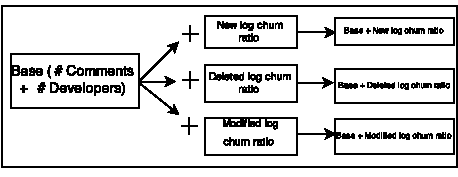
\includegraphics[width=8.8cm]{model}
	\caption{ Overview of our linear models for the resolution time of bugs }
	\label{fig:models}
\end{figure}

To better understand the usefulness of log churn on the time taken for fixing bugs, we build a linear regression model. Prior research has shown that resolution time is correlated to the number of developers and the number of comments in a issue report~\cite{RTpredictions}. We want to see whether the metrics from log churn (as shown in RQ1) can complement the number of developers and the number of comments in modelling the resolution time of bugs. The overview of the models is shown in Figure~\ref{fig:models}. We start with baseline model \textbf{BASE(\#comments+\#developers)} that uses the number of developers and the number of comments as independent variables~\cite{RTpredictions}. For the base model for each project, if the number of developers or the number of comments is not significant in the model, we remove the insignificant metric from the base model. We then build subsequent models in which we add our metrics that are measured in RQ1 as independent variables. The added metrics are $modified\ log\ churn\ ratio$, $new\ log\ churn\ ratio$, and $removed\ log\ churn\ ratio$. We add these metrics separately into the base model to examine whether each log churn related metric can complement the number of developers and the number of comments. We examine whether \DIFdelbegin \DIFdel{the }\DIFdelend each log churn related metric is significant in each model.

To measure the effect of each log churn related metric on the model, we follow a similar approach used in prior research~\cite{shihab,mocku}. We set all the metrics in the model to their means and find the predicted {\em`Resolution Time'}. Then we increase the metric of which we want to measure by one standard deviation value, while keeping the other metrics at their means. We then calculate the percentage of difference caused be increasing one of metrics by its standard deviation. A positive effect means a higher value of the log churn related metrics increases the {\em`Resolution Time'}, whereas a negative effect means that a higher value of the log churn related metrics  decreases the {\em`Resolution time'}.

We would like to point out that although linear regression has been used to build accurate models for the resolution time of bugs~\cite{RTpredictions}, our purpose of using the linear model in this paper is not for predicting the resolution time of bugs. Our purpose is to study the explanatory power of log churn related metrics and explore its empirical relation to the resolution time of bugs.%We controlled the metrics by total code churn. We used \textsl{Wilcoxon} test to measure the statistical significance of each metric in bugs fixed with log changes with bugs fixed without log changes. \textsl{Cohens.D} is used to measure the size of the difference of each metric. 



\subsubsection*{\textbf{Results}}

\textbf{We found that the logs are used to fix more complex bugs}. We find that the average code churn for fixing bugs is significantly higher with log churn than without log churn (see Table~\ref{tab:bugfixes} and Figure~\ref{fig:figure3}). Such results imply that developers may leverage logs to fix more complex bugs.

%This can be because (1) The information provided by existing logs is insufficient and hence they modify the logs to get additional data. (2) Developers are adding new methods or function and hence add logs to track the control and data flow in the new blocks.  

 
\begin{figure*}[thb]
	\centering
	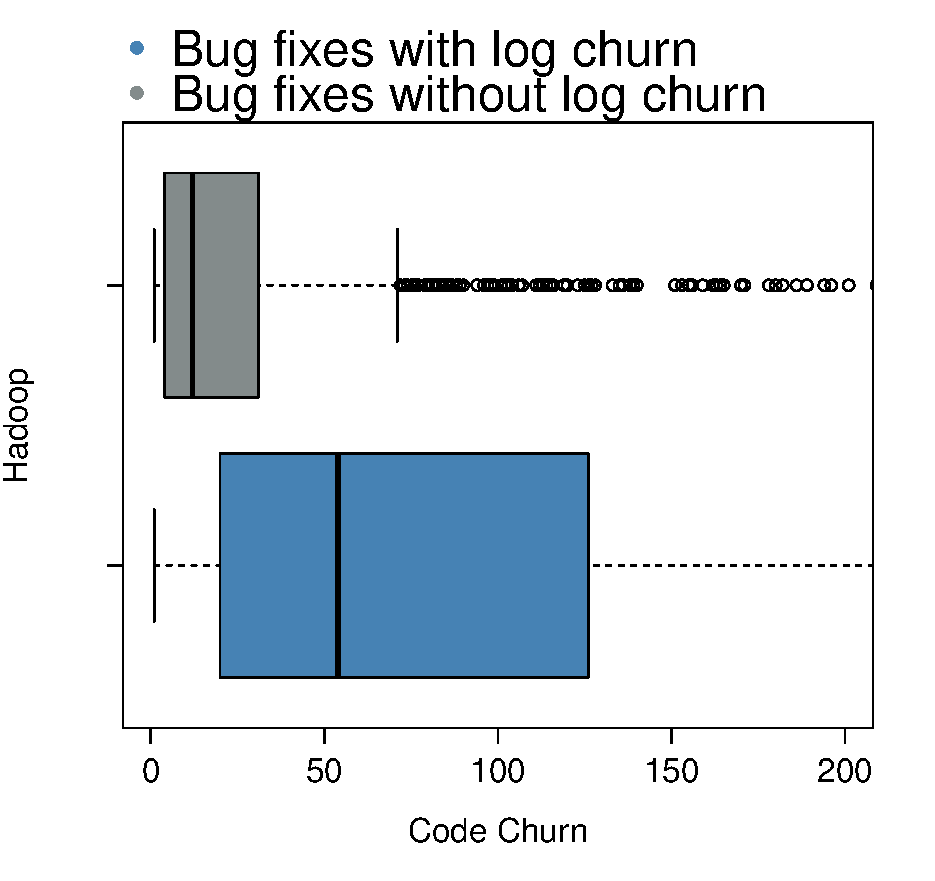
\includegraphics[width=.25\textwidth]{HadoopBoxPlot}
	\hfill
	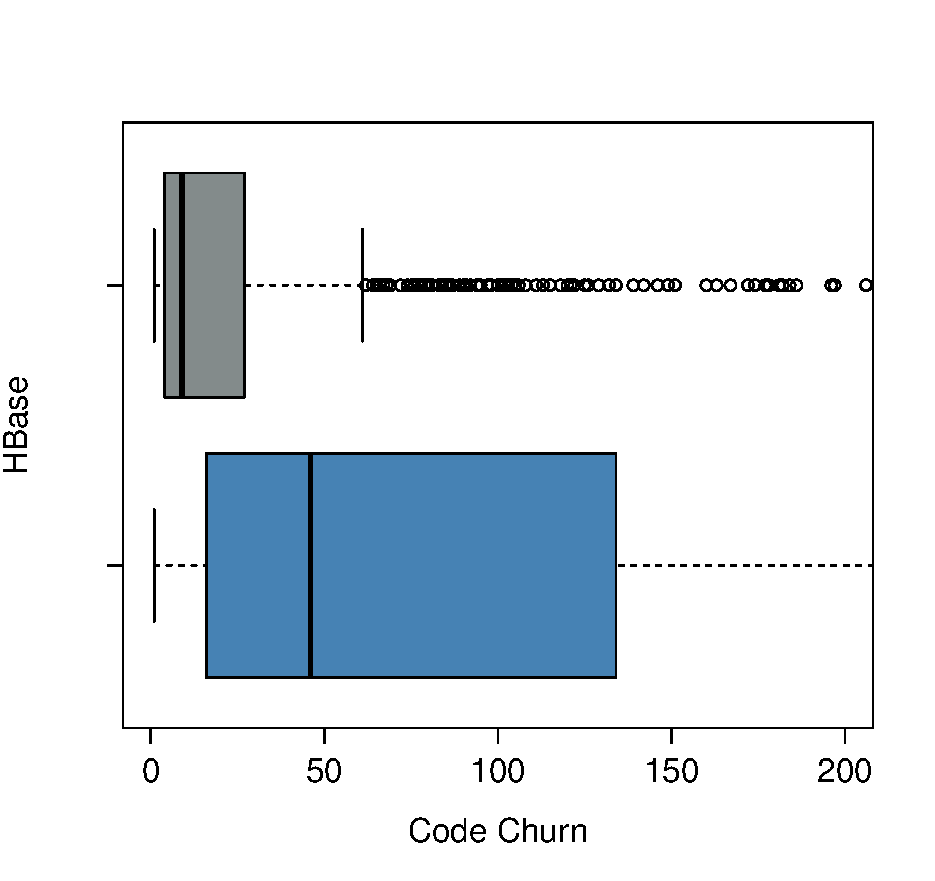
\includegraphics[width=.25\textwidth]{HBaseBoxPlot}\hfill
	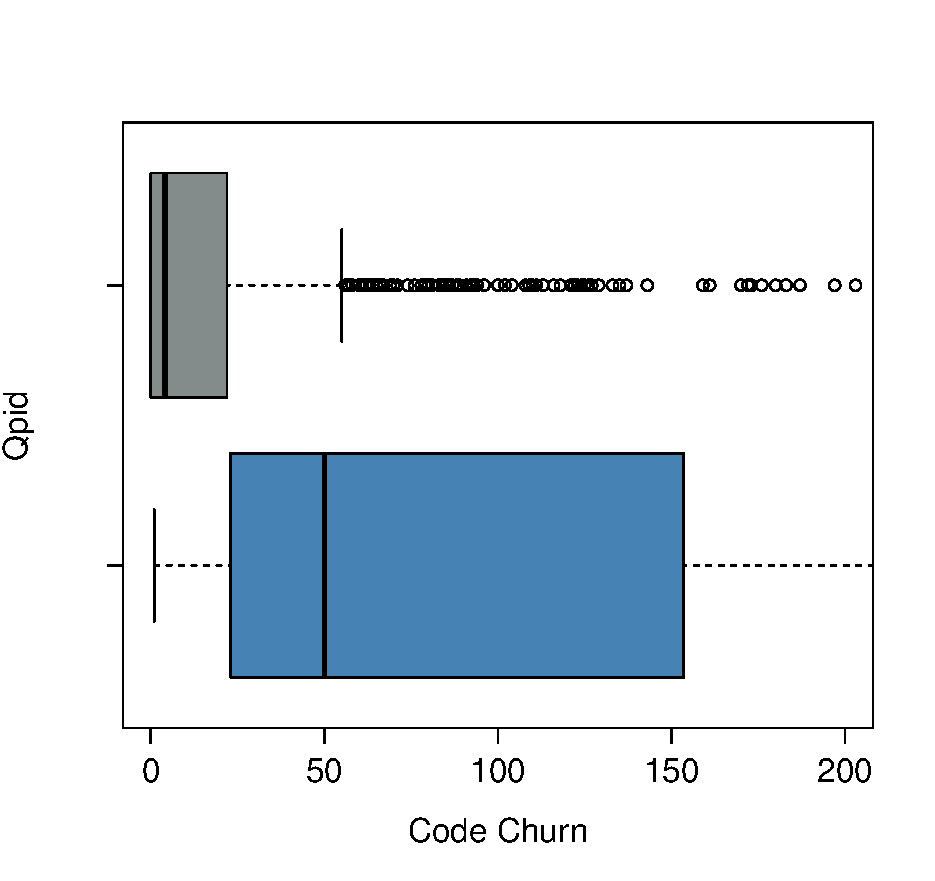
\includegraphics[width=.25\textwidth]{QpidBoxPlot}
	\caption{Boxplot of code churn of bug fixing commits with log churn (shown in blue) against bug fixing commits without log churn (shown in grey).}
	\label{fig:figure3}

\end{figure*}



\textbf{We found that bugs that are fixed with log churn take a shorter time with fewer comments and fewer people.} After controlling for code churn, we find that the resolution time, the number of comments and the number of developers are all statistically significantly smaller in the bug fixes with log churn than the ones without log churn. This result means that given two bugs of same complexity, the one with log churns takes less time to
get resolved and needs fewer number of developers involved with fewer discussions. This implies that logs provide useful information to assist developers in discussing, diagnosing and fixing bugs. For example, when fixing issue HBASE-3074 (commit 1,005,714), developers left the first comment to provide additional details in the logging message about where the failure occurs. In the source code, developers add the name of the servers into the the logging statements. This additional data helps trace the cause of the failure and helps in fixing the bug.  


\textbf{Log churn related metrics are significant in modelling the resolution time of bugs with negative effect.} From table~\ref{tab:logmetric} shows the effect of log churn related metrics when modeling resolution time. We find that the $new\ log\ churn\ ratio$ is significant in Hadoop and HBase when modelling resolution time of bug fixes and the $modified\ log\ churn\ ratio$ is significant in modelling the resolution time of bugs for Hadoop. Such results shows that there exists a relationship between log churns and the resolution time of bug fixes. We find that all log churn related metrics have negative effects on the resolution time of bugs. The negative effect implies that  more the developers leverage logs, the lesser time it takes for them to fix the bug. \DIFaddbegin \DIFadd{This is a important correlation and should not be confused with causation. }\DIFaddend 



\begin{table}[tbh]
	\caption{Effect of log churn related metrics on resolution time of bugs. Effect is measured by adding one standard deviation to its mean value, while the other metrics are kept at their mean values. The bold font indicates that the metric is statistically significant}
	\label{tab:logmetric}
	\centering{}%
	\begin{tabular}{|>{\centering}p{1.7cm}|>{\centering}p{1.7cm}|>{\centering}p{1.7cm}|>{\centering}p{1.7cm}|}
		\hline 
		Projects  & Hadoop & HBase & Qpid\tabularnewline
		\hline 
		\hline 
		new log churn ratio & \textbf{-4.55} {*}{*} & \textbf{-5.06 }{*}{*} & \textbf{-6.00}{ $\diamond$ } \tabularnewline
		\hline 
		removed log churn ratio & -3.24 & -4.16 & 	-2.37\tabularnewline
		\hline 
		modified log churn ratio & \textbf{-5.31} {*} & -3.7 & -6.31\tabularnewline
		\hline 
		\multicolumn{4}{c}{ *** p $<$ 0.001, ** p $<$  0.01, * p $<$  0.05,  $\diamond$ p $<$  0.1}\tabularnewline

		
	\end{tabular}	
\end{table}


\hypobox{Logs are  leveraged during fixing more complex bugs. Bug fixes with log changes are resolved faster with fewer people and fewer discussions. Log churn related metrics can complement number of comments and the number of developers in modelling the resolution time of bugs with a negative effect. Such results imply that there is a relationship between leveraging logs and a faster resolution of bugs.}


%
%Because there is less developers involved in the discussion, the number of discussions posts/comments on JIRA is also less. This is because when logs are leveraged, its easier to debug the problem so resolution time is less. Developer involvement is also less because, the bug can be traced and fixed easily and long discussions about root-cause analysis is avoided. 




%This example further validates our findings
%and shows that logs are indeed very useful in the debugging process.

%\hypobox{ Logs are leveraged during complex bugs and help in quicker resolution. 
%	Developers leverage logging statements to fix 	complex bugs. Bug fixes with log changes are resolved quicker with fewer people and less discussions. This implies provide useful information to fix bugs.	}

%\fbox{\begin{minipage}[t]{0.9\columnwidth}%
%\textbf{Findings}: From table 4, we find all metrics have negative effect sizes and are statistically significant.
%\textbf{Implication}: 
%This implies bugs without any log churn take
%longer to be fixed, need more involvement and discussions. This shows
%that logs play a vital role in solving bug fixes. Drawing from the
%manual study done in research question two, we observed that logs
%help in locating the buggy module and when fixes are made to the module,
%developers modify the logging statements. This is cyclic process and
%hence its vital that developers log in the initial development process.%
%\end{minipage}}

%
%To validate our study we did a manual study on to understand how logs
%are actually used in the debugging process. This is explained in further
%details in the subsequent section. 

%\subsection*{\textbf{RQ3: Does log churn impact resolution time of bug fixes? }}


\subsubsection*{\textbf{Motivation}}

In the previous research question we look at how logs are leveraged during bug fixes and if logs are useful during a bug fix. However, prior research has shown that resolution time is correlated to the number of developers and the number of comments in a issue report~\cite{RTpredictions}. In this RQ we explore if the log churn can increase the explanatory of the previous model and we study how each metric impacts the resolution time of bug fixes.

\subsubsection*{\textbf{Approach}}

We use logistic regression model, to study the explanatory power of our log churn metrics on resolution time. From previous studies we know that the number of developers and the number of  comments are effective in explaining resolution time~\cite {RTpredictions}. Therefore, we include these metrics along with our log churn metrics to increase the explanatory power of our model below,  

\begin{equation}
RT\ =  \alpha.Dev + \beta.Comm + \gamma.New + \theta.Del + \delta.Mod
\label{eq1}
\end{equation}

where $\alpha$, $\beta$, $\gamma$, $\theta$ and $\delta$ are the coefficients. 'Dev' is the number of developers involved in the fix, 'Comm' is the 	number of comments
% We start with baseline model and calculate the deviance explained to measure its explanatory power. We then add our log churn metrics to the baseline and compare the deviance explained by the newer model with baseline model. A higher percentage of deviance explained generally indicates a better model fit and higher explanatory power for the independent variables.


To understand the effect of each metric on the model we follow a similar approach used in prior research~\cite{shihab,mocku}. To measure the effect we set all the metrics in the model to their means and find the predicted probabilities. Then we increase the metric of which we want to measure by one standard deviation value, while keeping the other metrics at their means. We then calculate the percentage of difference caused be increasing one of metrics by its standard deviation. A positive effect means a higher value of the factor increases the likelihood, whereas a negative effect means that a higher value of the factor decreases the likelihood of the dependent variable.

We would like to point out that our purpose is not to predict the resolution time of bug fixes but to the impact of log churn metrics on resolution time of bug fixes.

\subsubsection*{\textbf{Results}} \textbf{We found that New Logs help in decreasing the resolution time of bug fixes}. From table~\ref{tab:logmetric} we see that 'New Log churn' are statistically significant in 2 of our subject systems and have negative effect on resolution time. This implies that new logs added during bugg fixing commit can help in reducing its resolution time. 

\textbf{Modifying logs has a negative impact on resolution of bug fix}. We observe that from table~\ref{tab:logmetric}, modified log churn has negative effect has negative effect in two subject systems and is statistically significant in Hadoop. This implies  modifying logs helps in fixing bugs faster. We observe that modified log churn is not significant in Hbase. This maybe because developers do not modify logs in Hbase as seen from table~\ref{tab:logchange}, where effect sizes are trivial for HBase.

We see that for new projects like Qpid, the source code is not well logged. So developers may add extra logs during complex bug fixes, increasing the resolution time bug fixes. This is seen in table~\ref{tab:logchange} where Qpid has the highest effect sizes among all projects for \textsl{'New Log churn'} and \textsl{'Modified Log churn'}, implying developers log extensively during bug fixes.

%\begin{table}
%		\protect\caption{Summary of metrics}
%		\hphantom{}
%		
%		\centering{}%
%\begin{tabular}{|>{\centering}p{1.7cm}|>{\centering}p{1.7cm}|>{\centering}p{1.7cm}|>{\centering}p{1.7cm}|}
%	\hline 
%	Projects  & Hadoop & Hbase & Qpid\tabularnewline
%	\hline 
%	\hline 
%	Base & 0.162 & 0.210 & 0.102\tabularnewline
%	\hline 
%	Base + New Log & 0.166 (+2.4\%){*}{*} & 0.212 (+1.0\%){*}{*} & 0.105 (+2.74)\tabularnewline
%	\hline 
%	Base + 	Deleted Log & 0.162 (0\%) & 0.210(0\%) & 0.102 (0\%)\tabularnewline
%	\hline 
%	Base + 	Modified Log & 0.162 (0\%){*} & 0.210 (0\%) & 0.105 (+2.7\%)\tabularnewline
%	\hline 
%	
%
%\end{tabular}
%\end{table}
%




\begin{table}
	\protect\caption{Effect of log churn metrics metrics on resolution time of bug fixes. Effect is measured by adding one standard deviation to its mean value, while the other metrics are kept at their mean values. The bold font indicates that the metric is statistically significant}
	\hphantom{}
	\label{tab:logmetric}
	\centering{}%
	\begin{tabular}{|>{\centering}p{1.7cm}|>{\centering}p{1.7cm}|>{\centering}p{1.7cm}|>{\centering}p{1.7cm}|}
	\hline 
	Projects  & Hadoop & Hbase & Qpid\tabularnewline
	\hline 
	\hline 
	New Log Churn & \textbf{-1.05} {*}{*} & \textbf{-1.26 }{*}{*} & 1.46 \tabularnewline
	\hline 
	Deleted Log Churn & -1 & -1.11 & 	0.84\tabularnewline
	\hline 
	 Modified Log Churn & \textbf{-0.6} {*} & -0.6 & 1.25\tabularnewline
	\hline
	\multicolumn{4}{c}{ *** p $<$ 0.001, ** p $<$  0.01, * p $<$  0.05, . p $<$  0.1}\tabularnewline

	
\end{tabular}



\end{table}





\DIFdelbegin \section{\DIFdel{A Manual Study on Leveraging Logs During Bug Fixes}}
%DIFAUXCMD
\addtocounter{section}{-1}%DIFAUXCMD
%DIFDELCMD < \label{sec:Manual}
%DIFDELCMD < %%%
\DIFdel{From the results of our research questions, we find that logs are often changed during  bug fixes and the bugs with log changes are fixed faster. However, from our data analysis, we do not know whether the changed logs are actually leveraged for bug fixes. }%DIFDELCMD < 

%DIFDELCMD < 
%DIFDELCMD < %%%
\DIFdel{To further study whether logs are leveraged during bug fixes, we perform a manual analysis to find out whether logs are leveraged during bug fixes. Where and what information provided by logs are used in bug fixes. We first collect all the issue reports with log churn. We then select a random sample from all the issue reports (180 samples) with 95}%DIFDELCMD < \% %%%
\DIFdel{confidence level and 5}%DIFDELCMD < \% %%%
\DIFdel{confidence interval. We read the discussion in each bug report to examine whether and how are log used in fixing the bug.}%DIFDELCMD < 

%DIFDELCMD < %%%
%DIF < \subsection*{\textbf{How often are logs leveraged during bug fixes? } }

%DIFDELCMD < 

%DIFDELCMD < %%%
\DIFdel{\textbf{In 70.7\% of the manually examined issue reports, logs are leveraged for bug fixes}. We find that developers leverage logs in 128 of examined issue reports (e.g. HBASE-3741). After identifying a bug, developers often leverage logging statements to trace the cause of bugs. %DIF < We find that in the remaining 29.3\% of the issue reports, developers leverage the exceptions that are printed in logs (e.g. QPID-4312) to fix bugs. 
We want to note that, for the bug reports that do not leverage logs in the issue report, logs may  be used but not discussed in the issue report. 
}%DIFDELCMD < 

%DIFDELCMD < 
%DIFDELCMD < %%%
%DIF < \subsection*{\textbf{What types of information in logs do developers use to fix bugs?} }

%DIFDELCMD < 

%DIFDELCMD < %%%
\DIFdel{\textbf{In 61\% of the bug reports made use of both variable and textual part in the logging statements to resolve bugs}. We observe that developers output the system state, the server/connection name, time, and even object names in the logs. We find that such information are often added by after-thought of developers during bug fixes. For example, to fix HBASE-3832, developers identify the cause of the problem using the logs. However, they fail to identify the exact conditions that cause the bug. Therefore, developers add more information into logs in order to fix the bug. Our results confirm that the text and the variable in the logs do help developers fix bugs.}%DIFDELCMD < 

%DIFDELCMD < 
%DIFDELCMD < %%%
%DIF < 
%DIF < 
%DIF < 
%DIF < developers provide a system generated log dump on JIRA.
%DIF < We observe that developers draw many conclusions using the logs present
%DIF < and this helps in resolving the bug. In this particular example, developers
%DIF < used the time-stamp, region-servers and the sequence-id's present
%DIF < in the logs. We also observed that these commits were associated with
%DIF < higher code churn implying, developers need more information to fix
%DIF < more complex problems.

%DIFDELCMD < 

%DIFDELCMD < %%%
%DIF < \textbf{39 \% of the reports used only the log message themselves to diagnose
%DIF < the problem.} We observed that majority of these bugs (38 commits), were caused by the logs themselves.
%DIF < These issues were either trivial from typos (example - commit 1333321), haphazard logs (example - commit 1333321) to complex issues degrading performance (example - commit 999046).
%DIF < 

%DIFDELCMD < 

%DIFDELCMD < 
%DIFDELCMD < %%%
%DIF < \hypobox{\textbf 70\% of the issues leverage logs during bug fixes, out of which 61\% of the issues leverage both textual and variable parameters in a logging statement. This validates our findings and shows that logs are leveraged by developers extensively during bug fixes. }

%DIFDELCMD < 

%DIFDELCMD < %%%
%DIF < 
\DIFdelend \section{Related Work}
\label{sec:Related}
%In this section we look at (1) the different usage of logs in improving
%software quality, (2) the tools which help in logging (3) the manual
%sampled studies done so far on analysis and characterization of logs,
%%so we can compare the results from our empirical study. 
%%
%
%\subsection*{Log Analysis:}

% The purpose of this section is to highlight the research that shows
%logs are used in debugging process. This is related to our work because
%(1) we show that logs are used in all the processes of a software
%life cycle, (2) how logs are useful in the improving the quality of
%the software. 


%
%Most prior work on log analysis focuses on studying the usefulness of logs during testing and detecting anomalies in large scale systems. \textsl{Shang et al.}\cite{IanContextinformation} showed mining execution logs in Big Data Analytic (BDA) applications, helps in finding differences in behavior of the system under different tests. \textsl{Lou et al}\cite{JGLouMining}  showed log parameters help in detecting anomalies in large systems. Their experiments on Hadoop and CloudDB showed their approach could detect anomalies at finer granularity and provide insight to developers. \textsl{Fu et al}\cite{QFuanomaly} built a Finite State Automaton (FSA) using unstructured logs and to detect performance bugs. \textsl{Zhen et al} \cite{ZhenMing} also showed logs can detect performance bugs but used clone detection techniques to abstract the unstructured logs. There has been substantial work in also trying to bridge the gap between
%operators of the software system and developers by \textsl{Shang et al}\cite{IanGap}. This
%is crucial as logs act as mediators in this regard, as they help in
%providing the operational information for the mediators and for developers
%it helps them track the system flow. In a later work the author further explores how communicated information through
%through logs are changed often and 40\%-60\% can be avoided  \textsl{Shang et al}\cite{IanWCRE}.
%
%
%Study done by \textsl{Xu et al}\cite{ConsoleLogs} on Hadoop and Darkstar file systems show that console logs help identify system
%bugs. Using Principal Component Analysis (PCA) they detect
%the anomalies and provide visualizations with decisions trees to assist developers in debugging. \textsl{Shang et al}\cite{WCSEIan} found log related metrics complement traditional metrics and increase the explanatory power of defect proneness by 40\%. Also, the manual analysis done in this paper shows that logs 36\% of logs are used in filed debugging. 
%Instead of trying to show how at specific instances logs are useful, in our paper  we focused on conducting a empirical study to understand how logs are leveraged during bug fixes. 
%
%% This is similar to our work
%%because, we also use source code parsing in finding the logs. But
%instead of trying to build structured logs we try to classify them
%using levenshtein distances.

% Similar work has been done to show how mining execution logs in large systems can help  detect anomalies and ensure good load tests  \textsl{Malik et al}\cite{Automatic}. This paper  \textsl{Lou et al}\cite{JGLouMining} discuss how invariants, mined from console logs can help to detect anomalies in large systems. \textsl{Fu et al}\cite{QFuanomaly} shows analysis of unstructured logs helps in detecting performance bugs in Distributed systems. Tools have also been developed to diagnose failures by mining execution logs \textsl{Tan et al}\cite{TanSalsa}. 

%Work has been done on mining execution logs in Big Data Analytic (BDA)
%applications to find difference in behavior of the system, when tests
%are run on small testing data and actual real world data \cite{IanContextinformation}.
%Similar work has been done to show how mining execution logs in large
%systems can help in detecting anomalies and ensure good load tests
%\cite{Automatic}. In the paper execution logs are mined and event
%pair are formed. By finding patterns in these event pairs dominant
%behavior of the system is identified. Any event which does not follow
%this is tagged as anomaly and can be reported to the developers. These
%papers show that logs are not used only for the purpose of debugging
%but can assist a developer in a variety of tasks. 
%
%Research has been to detect anomalies by invariant mining\cite{JGLouMining}.
%This paper focuses on constructing structured logs from console logs.
%After construction and grouping of log messages, invariants are mined.
%Any log which violates a invariant is considered to be an anomaly.
%Unstructured log analysis has shown to be useful in detecting in even
%Distributed Systems Several \cite{QFuanomaly}. In the paper a finite
%state automaton is built and trained to automatically detect performance
%bugs in the system. These papers consider print messages and other
%unstructured logs to extract information. Then they cluster or categorize
%the logging messages into groups and logs which fall into this cluster
%are treated as anomalies. Tools have also been developed to analyze
%system logs to obtain state-machine view, control and data flow models
%and other related statistics. SALSA\cite{TanSalsa} helps in deriving
%failure diagnosis techniques and visualization for different workloads
%in Hadoop project by mining execution logs. In our study, though we
%use the same system software (Hadoop),we try to understand how logs
%can be useful in debugging and not on trying to find the bug itself. 




%\subsection*{Empirical studies on logs:}

%In this section we try and find out how developers log. Is it done
%manually or do developers use established logging libraries. From
%our work on studying logging libraries in the Apache foundation we
%know that Slf4j, Log4j and Jakarta common logging are the most used
%libraries for logging. This helps us to find the logging statements
%in our case studies. Additionally there are many tools which help
%developers in logging \cite{Yuan}. The authors conduct a manual analysis and find that logs help in understanding the control and data flow in bug fixes but do not contain all the information to conclusively answer why the bug occurs. The paper addresses this issue through a tool called 'Log Enhancer' to enhance existing logs by providing additional details in the logs. This was tested with earlier version
%of the software and it was observed that 95\% of logs added by the
%tool were added by developer\textquoteright s overtime. This paper
%highlighted that do not log all the details in the first deployment
%and modify the logs in later revisions. This conforms to our findings
%as well, as we found that developers modify logs during debugging
%than other software process. 

%
%\textsl{Fu et al}\cite{Fu1} in an empirical study showed that logs are used for assertion checks, return value checks, exceptions, logic-branching and observing key points. The results of the analysis was evaluated by professionals from
%the industry and F-score of over 95\% was achieved. Similar to this, \textsl{Yuan et al}\cite{Characterizinglogs}  characterized logging practices in open-source systems. He found that over 33\% of all log changes are after thoughts and logs are changed 1.8 times more than entire code. \textsl{Shang et al}\cite{IanIcesm} analysis email threads from 3 large open-source projects and explains the different types of development knowledge that are sought by practitioners from logging statements. 



%Research has also been done to understand
%the needs of operators and administrators \cite{IanIcesm}. In this
%paper, by manually analyzing email threads in three large open-source
%projects, the authors find 5 different types of development knowledge
%that are sought by practitioners from logging statements. 
%add Sherbroke !!!!! -- ###
%
%\begin{figure*}
%	\centering
%	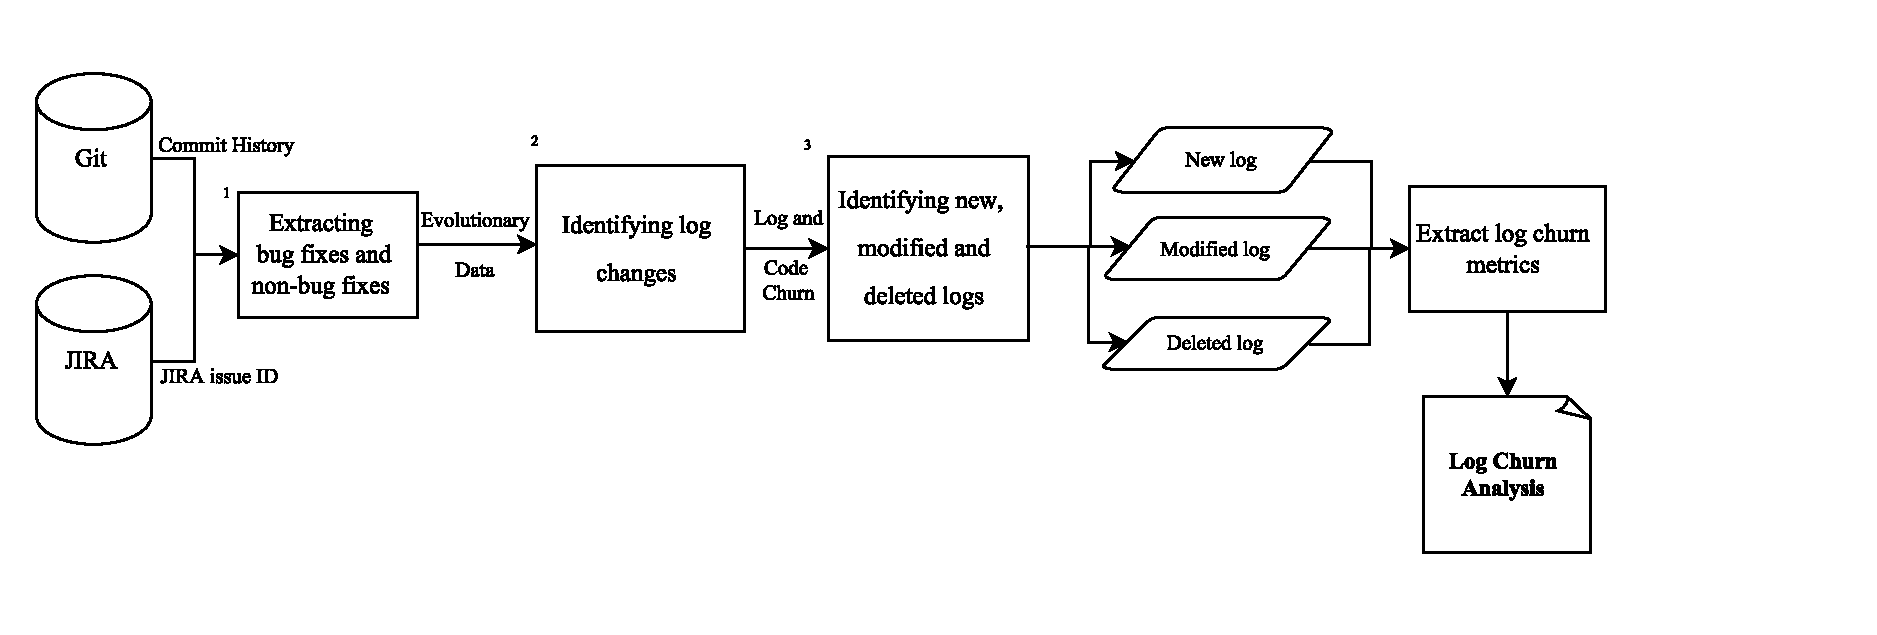
\includegraphics{MethdologyICESEM}
%	\caption{ Overview of our cast study approach }
%	\label{fig:MethodologyICSME}
%%\end{figure*}
%

%
%
%We finally look at other research work where logging practices have
%been analyzed to find where logs have been useful. Logs have been
%characterized in open-source systems and it has been shown that developers
%take multiple attempts to write correct log messages\cite{Characterizinglogs}.
%In this this paper, authors found that logs are actively maintained,
%they are changed more often and can help in diagnosing production-run
%failures. Our paper explores similar aspects, but we try to understand
%how logs are useful in debugging process in particular.
%
%Similar to the previous paper research has been done to study the
%logging practices in Industry \cite{Fu1}. This paper identified the
%most common places developers places logs in Industry. They found
%5 places where developers use logs and found the reasoning behind
%these decisions. The results were evaluated by professionals from
%the industry and F-score of over 95\% was achieved in predicting where
%logs are written. 


%Other studies have looked at the how logs change in large scale systems
%and how the information conveyed by these logs change over time \cite{IanWCRE}.
%In this paper the author explores how communicated information through
%through logs are changed often and 40\%-60\% can be avoided. It also
%shows, that CI with implementation details are changed more often. 

% \cite{Yuan}. The authors conduct a manual analysis and find that logs help in understanding the control and data flow in bug fixes but do not contain all the information to conclusively answer why the bug occurs. The paper addresses this issue through a tool called 'Log Enhancer' to enhance existing logs by providing additional details in the logs. This was tested with earlier version

In this section, we present the \DIFdelbegin \DIFdel{related work of this paper. In particular, we present the }\DIFdelend prior research that performs log analysis \DIFdelbegin \DIFdel{to for }\DIFdelend \DIFaddbegin \DIFadd{on }\DIFaddend large software systems and empirical studies \DIFaddbegin \DIFadd{done }\DIFaddend on logs. 


\subsection{Log Analysis}

% The purpose of this section is to highlight the research that shows
%logs are used in debugging process. This is related to our work because
%(1) we show that logs are used in all the processes of a software
%life cycle, (2) how logs are useful in the improving the quality of
%the software. 

Prior work leverage log analysis for testing and detecting anomalies in large scale systems. \textsl{Shang et al.}~\cite{IanContextinformation} propose an approach to leverage logs in verifying the deployment of Big Data Analytic applications. Their approach analyzes logs in order to find differences between running in a small testing environment and a large field environment. \textsl{Lou et al.}~\cite{JGLouMining} propose an approach to leverage variable values printed in logs to detect anomalies in large systems. Based on the variable values in logs, their approach creates invariants (e.g., equations). Any new logs that violates the invariant are considered to be a \DIFdelbegin \DIFdel{a }\DIFdelend sign of anomalies. \textsl{Fu et al}~\cite{QFuanomaly} built a Finite State Automaton (FSA) using unstructured logs and to detect performance bugs in distributed systems. 
\textsl{Xu et al}~\cite{ConsoleLogs} link logs to logging statements in source code to recover the text and and the variable parts of log messages. They applied Principal Component Analysis (PCA) to detect system anomalies. Tan et al.~\cite{TanSalsa} propose a tool named SALSA, which constructs state-machines from logs. The state-machines are further used to detect anomalies in distributed computing platforms. Jiang et al.~\cite{Jiang:2009:UCP:1525908.1525912} study the leverage of logs in troubleshooting issues from storage systems. They find that logs assist in a faster resolution of issues in storage systems. Beschastnikh et al.~\cite{Beschastnikh:2011:LEI:2025113.2025151, Beschastnikh:2014:IMC:2568225.2568246} designed automated tools that infers execution models from logs. These models can be used by developers to understand the behaviours of concurrent systems. Moreover, the models also assist in verifying the correctness of the system and fixing bugs.
To assist in fixing bugs using logs, Yuan \emph{et al$.$}~\cite{Yuan:2010:SED:1736020.1736038} propose an approach to automatically infer the failure scenarios when a log is printed during a failed run of a system.


\textsl{Jiang et al.}~\cite{Jiang:2008:AAA:1400155.1400158,JiangICSM2008, JiangICSM2009,Jiang:2010:ICS:1850000.1850068} proposed log analysis approaches to assist in automatically verifying results from load tests. Their log analysis approaches first automatically abstract logs into system events~\cite{Jiang:2008:AAA:1400155.1400158}. Based on the such events, they identified both functional anomalies~\cite{JiangICSM2008} and performance degradations~\cite{JiangICSM2009} in load test results. In addition, they proposed an approach that leverage logs to reduce the load test that are performed in user environment~\cite{Jiang:2010:ICS:1850000.1850068}.

The extensive prior research of log analysis motivate our paper to study how logs are leveraged during bug fixes. Our findings \DIFdelbegin \DIFdel{confirms }\DIFdelend \DIFaddbegin \DIFadd{also show }\DIFaddend that logs are \DIFdelbegin \DIFdel{widely leveraged }\DIFdelend \DIFaddbegin \DIFadd{leveraged more }\DIFaddend during bug fixes and the use of logs assists developers in a faster resolution of logs with fewer people and less discussion involved.



% This is similar to our work
%because, we also use source code parsing in finding the logs. But
%instead of trying to build structured logs we try to classify them
%using levenshtein distances.

% Similar work has been done to show how mining execution logs in large systems can help  detect anomalies and ensure good load tests  \textsl{Malik et al}\cite{Automatic}. This paper  \textsl{Lou et al}\cite{JGLouMining} discuss how invariants, mined from console logs can help to detect anomalies in large systems. \textsl{Fu et al}\cite{QFuanomaly} shows analysis of unstructured logs helps in detecting performance bugs in Distributed systems. Tools have also been developed to diagnose failures by mining execution logs \textsl{Tan et al}\cite{TanSalsa}. 

%Work has been done on mining execution logs in Big Data Analytic (BDA)
%applications to find difference in behavior of the system, when tests
%are run on small testing data and actual real world data \cite{IanContextinformation}.
%Similar work has been done to show how mining execution logs in large
%systems can help in detecting anomalies and ensure good load tests
%\cite{Automatic}. In the paper execution logs are mined and event
%pair are formed. By finding patterns in these event pairs dominant
%behavior of the system is identified. Any event which does not follow
%this is tagged as anomaly and can be reported to the developers. These
%papers show that logs are not used only for the purpose of debugging
%but can assist a developer in a variety of tasks. 
%
%Research has been to detect anomalies by invariant mining\cite{JGLouMining}.
%This paper focuses on constructing structured logs from console logs.
%After construction and grouping of log messages, invariants are mined.
%Any log which violates a invariant is considered to be an anomaly.
%Unstructured log analysis has shown to be useful in detecting in even
%Distributed Systems Several \cite{QFuanomaly}. In the paper a finite
%state automaton is built and trained to automatically detect performance
%bugs in the system. These papers consider print messages and other
%unstructured logs to extract information. Then they cluster or categorize
%the logging messages into groups and logs which fall into this cluster
%are treated as anomalies. Tools have also been developed to analyze
%system logs to obtain state-machine view, control and data flow models
%and other related statistics. SALSA\cite{TanSalsa} helps in deriving
%failure diagnosis techniques and visualization for different workloads
%in Hadoop project by mining execution logs. In our study, though we
%use the same system software (Hadoop),we try to understand how logs
%can be useful in debugging and not on trying to find the bug itself. 



\subsection{Empirical studies on logs}

%In this section we try and find out how developers log. Is it done
%manually or do developers use established logging libraries. From
%our work on studying logging libraries in the Apache foundation we
%know that Slf4j, Log4j and Jakarta common logging are the most used
%libraries for logging. This helps us to find the logging statements
%in our case studies. Additionally there are many tools which help
%developers in logging \cite{Yuan}. The authors conduct a manual analysis and find that logs help in understanding the control and data flow in bug fixes but do not contain all the information to conclusively answer why the bug occurs. The paper addresses this issue through a tool called 'Log Enhancer' to enhance existing logs by providing additional details in the logs. This was tested with earlier version
%of the software and it was observed that 95\% of logs added by the
%tool were added by developer\textquoteright s overtime. This paper
%highlighted that do not log all the details in the first deployment
%and modify the logs in later revisions. This conforms to our findings
%as well, as we found that developers modify logs during debugging
%than other software process. 

Prior research \DIFdelbegin \DIFdel{has performed empirical studied }\DIFdelend \DIFaddbegin \DIFadd{performs an empirical study  }\DIFaddend on logs and logging characteristics. Yuan et al.~\cite{Characterizinglogs} studies the logging characteristics in four open source systems. They find that over 33\% of all log changes are after thoughts and logs are changed 1.8 times more than entire code. Fu \textsl{et al$.$}~\cite{Fu1} performed an empirical study on where developer put logging statements. They find that logging statements are used for assertion checks, return value checks, exceptions, logic-branching and observing key points. The results of the analysis \DIFdelbegin \DIFdel{was }\DIFdelend \DIFaddbegin \DIFadd{were }\DIFaddend evaluated by professionals from the industry and F-score of over 95\% was achieved. 


\textsl{Shang et al.}~\cite{IanGap} signify the fact that there is gap between operators and developers of software systems, especially in the leverage of logs. They performed an empirical study on the evolution both static logging statements and log lines outputted during run time~\cite{EMSEIAN, SMR:SMR1579}. They find that logs are co-evolving with the software systems. However, logs are often modified by developers without considering the needs of operators. Furthermore, \textsl{Shang et al}~\cite{IanIcesm} find that understanding logs is challenging. They examine user mailing lists from three large open-source projects and find that users of these systems have various issues in understanding logs. \textsl{Shang et al.} propose to leverage different types of development knowledge, such as issue reports, to assist in understanding logs. 

Prior research by \textsl{Yuan et al.}~\cite{Yuan} shows that logs need to be improved by providing additional information. Their tool named \emph{Log Enhancer} can automatically \DIFdelbegin \DIFdel{provides }\DIFdelend \DIFaddbegin \DIFadd{provide }\DIFaddend additional control and data flow parameters into logs. 

The most related prior research by Shang \emph{et al$.$}~\cite{EMSEIAN} empirically study the relationship of logging practice and code quality. Their manual analysis sheds \DIFdelbegin \DIFdel{some lights }\DIFdelend \DIFaddbegin \DIFadd{light }\DIFaddend on the fact that some logs are changed due to field debugging. They also show that there is a strong relationship between  logging practice and code quality. Our paper focused on understanding how logs are leveraged during bug fixes. Our results show that logs are  leveraged extensively during bug fixes and assist in a quick resolution of bugs. 





%Research has also been done to understand
%the needs of operators and administrators \cite{IanIcesm}. In this
%paper, by manually analyzing email threads in three large open-source
%projects, the authors find 5 different types of development knowledge
%that are sought by practitioners from logging statements. 
%add Sherbroke !!!!! -- ###

%
%
%We finally look at other research work where logging practices have
%been analyzed to find where logs have been useful. Logs have been
%characterized in open-source systems and it has been shown that developers
%take multiple attempts to write correct log messages\cite{Characterizinglogs}.
%In this this paper, authors found that logs are actively maintained,
%they are changed more often and can help in diagnosing production-run
%failures. Our paper explores similar aspects, but we try to understand
%how logs are useful in debugging process in particular.
%
%Similar to the previous paper research has been done to study the
%logging practices in Industry \cite{Fu1}. This paper identified the
%most common places developers places logs in Industry. They found
%5 places where developers use logs and found the reasoning behind
%these decisions. The results were evaluated by professionals from
%the industry and F-score of over 95\% was achieved in predicting where
%logs are written. 


%Other studies have looked at the how logs change in large scale systems
%and how the information conveyed by these logs change over time \cite{IanWCRE}.
%In this paper the author explores how communicated information through
%through logs are changed often and 40\%-60\% can be avoided. It also
%shows, that CI with implementation details are changed more often. 

% \cite{Yuan}. The authors conduct a manual analysis and find that logs help in understanding the control and data flow in bug fixes but do not contain all the information to conclusively answer why the bug occurs. The paper addresses this issue through a tool called 'Log Enhancer' to enhance existing logs by providing additional details in the logs. This was tested with earlier version


%We also know logging practices can also assess the code quality of
%platform software \cite{WCSEIan}. This paper showed that logging
%characteristics can help in predicting defect prone modules in software,
%as developers tend to log more when they feel a module has a higher
%chance to be prone to bugs. This paper looked at Hadoop and Jboss
%and found log related metrics complement traditional metrics and increase
%the explanatory power of defect proneness by 40\%. The other imortant
%aspect of this paper is the manual analysis done to identify the different
%reasons being logging statements. We did similar manual analysis in
%our paper to find the types of logging changes that occur (section
%4.2) and to understand the different usage of logs in debugging (section
%5).
%
%All this prior work tries to look at usage of logs from different
%perspectives but none of them attempt to measure if logs are actually
%helpful in the development process, especially in debugging. Some
%of the work is done through manual analysis and has not been done
%on different systems to verify the results.

%platform software \cite{WCSEIan}. This paper showed that logging
%characteristics can help in predicting defect prone modules in software,
%%as developers tend to log more when they feel a module has a higher
%chance to be prone to bugs. This paper looked at Hadoop and Jboss
%and found log related metrics complement traditional metrics and increase
%the explanatory power of defect proneness by 40\%. The other imortant
%aspect of this paper is the manual analysis done to identify the different
%reasons being logging statements. We did similar manual analysis in
%our paper to find the types of logging changes that occur (section
%4.2) and to understand the different usage of logs in debugging (section
%5).
%
%All this prior work tries to look at usage of logs from different
%perspectives but none of them attempt to measure if logs are actually
%helpful in the development process, especially in debugging. Some
%of the work is done through manual analysis and has not been done
%on different systems to verify the results.




\section{Limitations and Threats to Validity}
\label{sec:Limit}

In this section, we present the threats to the validity to our findings.

\subsection*{External Validity}


Our study is performed  \DIFdelbegin \DIFdel{and }\DIFdelend Hadoop, HBase and Qpid. Even though \DIFaddbegin \DIFadd{these }\DIFaddend three subject systems have years of history and large user bases, the three subject systems are all \DIFdelbegin \DIFdel{based on Java }\DIFdelend \DIFaddbegin \DIFadd{Java based platform systems}\DIFaddend . More case studies on other software in other domains with other programming languages are needed to see whether our findings can be generalized. 


%The other limitation is projects in which logging data is less. We
%ran experiments on several other projects like Cassandra, Cayene,
%Zookeeper and Lucene. In all these projects the total number of logging
%statements were less to draw any meaningful conclusions. When we manually
%examined the data for Cassandra and Lucene we observed many custom
%logging statements which were not caught from pattern matching. As
%stated above its almost impossible to catch all instances of these
%custom logs in projects.


\subsection*{Internal Validity}


Our study is based on the data obtained from SVN and JIRA for all the subject systems. The
quality of the data contained in the repositories can impact the internal validity of
our study.

Our analysis of the relationship between logs and bug resolution time cannot claim causal effects, as we
are investigating correlations, rather than conducting impact studies. The explanative power of log churn related metrics on the resolution time of bugs does not indicate that logs cause faster resolution of bugs. Instead, it indicates the possibility of a relation that should be studied in
depth through user studies.



\subsection*{Construct Validity}

The heuristics to extract logging source code may not be able to extract every logging statement in the source code. Even though the subject systems leverage logging libraries to generate logs at runtime, there still exist user-defined logging statements. By manually examining the source code, we believe that we extract most of the logging statements. Evaluation on the coverage of our extracted logging statements can address this threat.

We use keywords to identify bug fixing commits when the JIRA issue id is not included in the commit messages. We also use \DIFdelbegin \DIFdel{keyword }\DIFdelend \DIFaddbegin \DIFadd{keywords }\DIFaddend to identify branching and merging commits. Although such \DIFdelbegin \DIFdel{keyword }\DIFdelend \DIFaddbegin \DIFadd{keywords }\DIFaddend are used extensively in prior research~\cite{EMSEIAN}, we may still miss identify bug fixing commits or branching and merging commits. 

We  use Levenshtein distance and choose a threshold to identify log modification. However, such threshold may not accurately identify log modification. Further sensitivity analysis on such threshold is needed to better understand the impact of the threshold to our findings.

We build a linear regression to model the resolution time of bugs. However, the relationship between log churn and the resolution time of bugs may not be linear. In addition, there may exist interactions between metrics. For example, the logs in debug logging level may have a higher relationship with the resolution time of bugs. However, as the first exploration of the leverage of logs in bug fixes, we only use linear model to find out whether the leverage of logs have a relationship with the resolution time of bugs. The resolution time of bugs can be correlated to many factors other than just logs, such as the complexity of code fixes. To reduce such a possibility, we control the log churn related metrics by code churn. However, other factors may also have an impact on the resolution time of bugs. Future studies should build more complex models that consider these other factors.


Source code from different components of a system may have various characteristics. The importance of logs in bug fixes may vary in different components of the subject systems. More empirical studies on the use of logs in fixing bugs for different components of the systems are needed.



%
%commits which has type Branching in them and removed these
%branching commits from our data set. But we later found some of the
%commits are tagged under the category of UNKNOWN. When its under 'Unknown'
%category it was impossible to know if its branching or not. 

\section{Conclusion and Future Work}
\label{sec:Conclusion}
%
%
%Logs are used by developers for finding anomalies, monitor performance, software maintenance, capacity planning and also in debugging errors. Our paper presents a empirical study of log leverage during bug fixes. Using three subject systems (Hadoop, HBase and Qpid) we understand how logs are leveraged, the different types of log changes developers make and if logs are useful in the debugging process.
%We find that logs are leveraged more during bug fixing commits by developers. In particular we find logs are modified and new logs are added during bug fixing commits. This means existing logs do not convey all the information for fixing the bug and have to be modified or new logs added. We find four different types of log modifications namely change to  `Text Modification',
%`Variable Changes', `Log Relocating' and `Logging Level Changes'. Of these four types, we find developers modify variables more. This implies that developers require more specific data to fix bugs and leverage logs to collect it. We also find that developers leverage logs during complex bug fixes, where complexity is measured using total churn of a commit. We find that bug fixes which leverage logs are resolved quicker, need fewer developers and less discussions. From the linear model built we find that adding new logs and modifying logs has negative  impact on the resolution time of bug fixes. These results imply there is a relationship between leveraging logs and a faster resolution of bugs.
%\indent Finally we did a manual analysis were we find developers use logging statements to understand the rationale behind logs. We find in over 70 \% of the bug fixing issues, developers used logs in the debugging process. We also find that in over 61 \% of the bug fixing  issues, developers leverage both the contextual and variable information in logging statements to fix the bug.
%
%Though its known logs are useful, our research presents the first empirical study on log leverage during bug fixes.	Our study demonstrates the importance of logging during bug fixes and shows developers that logs are useful in faster resolution of bugs.



Logs are used by developers for finding anomalies, monitor performance, software maintenance, capacity planning and also in fixing bugs. The leverage of logs and their usefulness during bug fixes has never been empirically studied before. This paper is a first attempt (to our best knowledge) to understand whether and how are logs leveraged during bug fixes. The highlights of our findings are:

\begin{itemize}
	\item We find that logs are used more during bug fixing commits. In particular, we find logs are modified more frequently during bug fixes. More specifically we find that variables and textual information in the logs are more frequently modified during bug fixes. 
	\item We find that logs are leveraged in fixing more complex bugs. However, bug fixes that leverage logs are faster, need fewer developers and have less discussion.
	\item We find that log modification and new logs are significant in modeling the resolution time of bugs. More the log modification or addition of new logs, the shorter the resolution time of bugs. 
\end{itemize} 

Our findings show that logs are used extensively by developers in bug fixes and logs are useful during bug fixes. We find that developers modify the text or variables in logging statements frequently as after-thoughts during bug fixes. This suggests that software developers should allocate more effort for considering the text, the printed variables in the logging statements when developers first add logging statements to the source code. Hence, bugs can be fixed faster without the necessity to change logs during the fix of bugs. 



%Our findings do not advocate the removal of logs that are a critical instrument used
%by developers to understand and monitor the field quality of their software. Instead,
%our findings suggest that software maintainers should allocate more preventiveEmpir Software Eng
%maintenance effort on source code files with more logs and log churn, since such
%source code files might be the ones where developers and operators may have more
%doubts and concerns, and hence are more defect prone.

% An example of a floating figure using the graphicx package.
% Note that \label must occur AFTER (or within) \caption.
% For figures, \caption should occur after the \includegraphics.
% Note that IEEEtran v1.7 and later has special internal code that
% is designed to preserve the operation of \label within \caption
% even when the captionsoff option is in effect. However, because
% of issues like this, it may be the safest practice to put all your
% \label just after \caption rather than within \caption{}.
%
% Reminder: the "draftcls" or "draftclsnofoot", not "draft", class
% option should be used if it is desired that the figures are to be
% displayed while in draft mode.
%
%\begin{figure}[!t]
%\centering
%\includegraphics[width=2.5in]{myfigure}
% where an .eps filename suffix will be assumed under latex, 
% and a .pdf suffix will be assumed for pdflatex; or what has been declared
% via \DeclareGraphicsExtensions.
%\caption{Simulation results for the network.}
%\label{fig_sim}
%\end{figure}

% Note that IEEE typically puts floats only at the top, even when this
% results in a large percentage of a column being occupied by floats.


% An example of a double column floating figure using two subfigures.
% (The subfig.sty package must be loaded for this to work.)
% The subfigure \label commands are set within each subfloat command,
% and the \label for the overall figure must come after \caption.
% \hfil is used as a separator to get equal spacing.
% Watch out that the combined width of all the subfigures on a 
% line do not exceed the text width or a line break will occur.
%
%\begin{figure*}[!t]
%\centering
%\subfloat[Case I]{\includegraphics[width=2.5in]{box}%
%\label{fig_first_case}}
%\hfil
%\subfloat[Case II]{\includegraphics[width=2.5in]{box}%
%\label{fig_second_case}}
%\caption{Simulation results for the network.}
%\label{fig_sim}
%\end{figure*}
%
% Note that often IEEE papers with subfigures do not employ subfigure
% captions (using the optional argument to \subfloat[]), but instead will
% reference/describe all of them (a), (b), etc., within the main caption.
% Be aware that for subfig.sty to generate the (a), (b), etc., subfigure
% labels, the optional argument to \subfloat must be present. If a
% subcaption is not desired, just leave its contents blank,
% e.g., \subfloat[].


% An example of a floating table. Note that, for IEEE style tables, the
% \caption command should come BEFORE the table and, given that table
% captions serve much like titles, are usually capitalized except for words
% such as a, an, and, as, at, but, by, for, in, nor, of, on, or, the, to
% and up, which are usually not capitalized unless they are the first or
% last word of the caption. Table text will default to \footnotesize as
% IEEE normally uses this smaller font for tables.
% The \label must come after \caption as always.
%
%\begin{table}[!t]
%% increase table row spacing, adjust to taste
%\renewcommand{\arraystretch}{1.3}
% if using array.sty, it might be a good idea to tweak the value of
% \extrarowheight as needed to properly center the text within the cells
%\caption{An Example of a Table}
%\label{table_example}
%\centering
%% Some packages, such as MDW tools, offer better commands for making tables
%% than the plain LaTeX2e tabular which is used here.
%\begin{tabular}{|c||c|}
%\hline
%One & Two\\
%\hline
%Three & Four\\
%\hline
%\end{tabular}
%\end{table}


% Note that the IEEE does not put floats in the very first column
% - or typically anywhere on the first page for that matter. Also,
% in-text middle ("here") positioning is typically not used, but it
% is allowed and encouraged for Computer Society conferences (but
% not Computer Society journals). Most IEEE journals/conferences use
% top floats exclusively. 
% Note that, LaTeX2e, unlike IEEE journals/conferences, places
% footnotes above bottom floats. This can be corrected via the
% \fnbelowfloat command of the stfloats package.





% conference papers do not normally have an appendix





% trigger a \newpage just before the given reference
% number - used to balance the columns on the last page
% adjust value as needed - may need to be readjusted if
% the document is modified later
%\IEEEtriggeratref{8}
% The "triggered" command can be changed if desired:
%\IEEEtriggercmd{\enlargethispage{-5in}}

% references section

% can use a bibliography generated by BibTeX as a .bbl file
% BibTeX documentation can be easily obtained at:
% http://www.ctan.org/tex-archive/biblio/bibtex/contrib/doc/
% The IEEEtran BibTeX style support page is at:
% http://www.michaelshell.org/tex/ieeetran/bibtex/
%\bibliographystyle{IEEEtran}
% argument is your BibTeX string definitions and bibliography database(s)
%\bibliography{IEEEabrv,../bib/paper}
%
% <OR> manually copy in the resultant .bbl file
% set second argument of \begin to the number of references
% (used to reserve space for the reference number labels box)


\bibliographystyle{IEEEtran}
\bibliography{Logreference}








% that's all folks
\end{document}


